\documentclass[12pt]{report}
\usepackage[top=23mm,bottom=23mm,left=23mm,right=23mm]{geometry}
\usepackage[dvipsnames]{xcolor}
\usepackage{fancyhdr, lastpage}
\usepackage{times}
\usepackage{chapterbib}
\usepackage[sectionbib]{natbib}
\bibpunct{(}{)}{;}{a}{,}{,}
\usepackage{graphicx}
\usepackage{epstopdf}
\usepackage{subfigure}
\usepackage[footnotesize, bf]{caption}
\usepackage{amsmath}
\usepackage{amssymb}
\usepackage{amsthm}
\usepackage{setspace}
\usepackage[small,compact]{titlesec}
\usepackage{multicol}
\usepackage{multirow}
\usepackage{wrapfig}
% \usepackage{minitoc}  Was not compatible with anything
\usepackage{array}
\usepackage{tikz}
\usetikzlibrary{matrix}
\usepackage{listings}
\usepackage{enumerate}  % for enumerating with a), b) etc...
\usepackage{caption}    % for having enumertion in a caption 
\usepackage{cleveref}   % So multiple references will auto format themself
\usepackage{algorithm2e}
%\usepackage{hyperref}   % This allows for hyperlinks in the table of content
%\hypersetup{
%  colorlinks,
%  citecolor=black,
%  filecolor=black,
%  linkcolor=black,
%  urlcolor=black
%}

\usepackage[mathlines]{lineno}  % Line numbers in document...
%% parameters for lineno to work nicely
\linenumbers

%% Supress annoying warnings
%\usepackage{silence}
%\WarningFilter{latex}{Text page}

\makeatletter
% Make a copy of macros responsible for entering display math mode
\let\start@align@nopar\start@align
\let\start@gather@nopar\start@gather
\let\start@multline@nopar\start@multline
% Add the "empty line" command to the macros
\long\def\start@align{\par\start@align@nopar}
\long\def\start@gather{\par\start@gather@nopar}
\long\def\start@multline{\par\start@multline@nopar}
\makeatother

%% Thereom and Proposition stuff
\theoremstyle{plain}
\newtheorem{thm}{Theorem}[section]
\newtheorem{prop}[thm]{Proposition}

%Folder paths that contain graphics
\graphicspath{
  {./}
  {Chapters/1_introduction/Figures/}
  {Chapters/3_numerics/Figures/}
  {Chapters/4_simulation/Figures/}
}

%\usepackage[colorlinks=true,linkcolor=blue]{hyperref}
% PDF hyper-linking (set colors to black for printing)
%\usepackage[ps2pdf=true,colorlinks]{hyperref}
%\usepackage[figure,table]{hypcap}
%\hypersetup{
%	bookmarksnumbered,
%	pdfstartview={FitH},
%	citecolor={black},
%	linkcolor={black},
%	urlcolor={black},
%	pdfpagemode={UseOutlines}
%}

\pdfinfo{
/Author (Eric M. Jalbert, 2015)
/Title (Comparison of Semi-Implicit and Fully-Implicit Time Integration Methods for a Highly Degenerate Diffusion-Reaction Equation Coupled with an ODE)
/Subject (Comparison of Semi-Implicit and Fully-Implicit Time Integration Methods for a Highly Degenerate Diffusion-Reaction Equation Coupled with an ODE)
}

%Paragraph symmetries...
\setlength{\parskip}{10pt}
\setlength{\parindent}{0pt}
\setlength{\parsep}{0pt}


\setcounter{secnumdepth}{5}
\setcounter{tocdepth}{1}
%\setcounter{minilofdepth}{2}
\renewcommand{\abstractname}{\Large ABSTRACT}
\renewcommand{\bibname}{References}
%\renewcommand\bibsection{}
%\renewcommand{\bibsep}{0pt}

\setlength{\headheight}{15pt}

\fancypagestyle{custom}{
\lhead{\textit{E.Jalbert, 2014}}
\rhead{\textit{COMPARISON SEMI- FULLY-IMPLICIT METHODS}}
}

\fancypagestyle{normal}{
\lhead{\textit{\rightmark}}
\rhead{\textit{\leftmark}}
}

\fancypagestyle{chp3-5}{
\lhead{\textit{3.5. COMPARE OF SEMI-FULLY-IMPLICIT METHODS}}
\rhead{\textit{CHAPTER 3. NUMERICAL METHODS}}
}

\fancypagestyle{References}{
\lhead{}
\rhead{\textit{REFERENCES}}
}

%%%%%%%%% If I have appendies, add the fancy page styles 
%%%%%%%%% like the example below
%\fancypagestyle{AppendixA}{
%\lhead{}
%\rhead{\textit{APPENDIX A: Default Simulation Parameters}}
%}

\begin{document}

%PreliminarySections
\pagenumbering{roman}
%----------------------------------------------------------
% Title Page
%   The first page of the thesis, contains 
%   author/university/title and other info
%----------------------------------------------------------
\begin{titlepage}
  \begin{center}
    \vspace*{4cm}
    \LARGE\large{Comparison of a Semi-Implicit and a Fully-Implicit Time Integration Method for a Highly Degenerate Diffusion-Reaction Equation Coupled with an Ordinary Differential Equation}
    \vspace*{0.5cm}
    
    \small{by}
    \vspace*{0.5cm}
    
    \large{Eric M. Jalbert}
    \vspace*{3.5cm}
    
    A Thesis\\presented to\\The University of Guelph
    \vspace*{1.5cm}
    
    In partial fulfilment of requirements\\for the degree of\\Master of Science\\in\\Applied Mathematics
    \vfill

    Guelph, Ontario, Canada
    
    $\copyright$ E.M. Jalbert, January, 2015
  \end{center}
\end{titlepage}






%Abstract
%\phantomsection
\addcontentsline{toc}{section}{Abstract}
%\section*{ABSTRACT}
\begin{abstract}
\setcounter{page}{2}
\begin{center}
%\vspace*{33pt}
\large{\textbf{Comparison of a Semi-Implicit and a Fully-Implicit Time Integration Method for a Highly Degenerate Diffusion-Reaction Equation Coupled with and Ordinary Differential Equation}}\\
\vspace*{20pt}
\begin{minipage}{0.49\textwidth}
\begin{flushleft}
\normalsize{Eric M. Jalbert}\\
\normalsize{University of Guelph,2015}
\end{flushleft}
\end{minipage}
\begin{minipage}{0.49\textwidth}
\begin{flushright}
\normalsize{Advisor}\\
\normalsize{Professor Hermann J. Eberl}
\end{flushright}
\end{minipage}
\end{center}
\vspace*{20pt}

A certain class of highly degenerate diffusion equations arises when modelling biofilm growth and propagations.
We focus on the cellulolytic \textit{Clostridium thermocellum}, because of its potential in the field of energy biotechnology.
From this system a spatially implicit model was proposed in the literature before.
Here we study a spatially explicit model.
In contrast to other biofilm systems, a special feature of this system is that the growth promoting nutrient is not diffusive but bound in the substratum on which the biofilm grows.
As a consequence one obtains a highly degenerate diffusion-reaction equation for the bacteria that is coupled to an ordinary differential equation for nutrients.
The degeneracy of the biomass equation introduces gradient blow-up at the interface which makes numerical treatment difficult.
For this, a fully-implicit time integration method is formulated so that it generalises a previously used semi-implicit method to solve the problem with increased accuracy.
The fully-implicit method uses, at each time-step, a fixed-point iteration to solve the arising nonlinear algebraic equation and can be controlled by the required tolerance for convergence.

This method is validated and tested to investigate numerous issues that arise with numerical computations: mass conservations, preservation of symmetries in the initial data, and convergence with respect to grid refinement.
Furthermore, a difference is quantified between the fully-implicit and the simpler semi-implicit methods which it generalises.
The trade-off between improved accuracy and increased computational effort is found to be optimal for tolerances that force a single extra iteration of the fully-implicit method.

The numerical method is then used to simulate \textit{C.thermocellum} biofilm formation on cellulose sheets with the main objectives of (i) understanding patterns of biofilm formation and (ii) understanding how including the spatial diffusion terms in the biomass affect the results of the simulations at a reactor-scale.
Our simulation results strongly suggest the formation of travelling wave solutions that describe how the biofilm moves across the substratum.
To test the effect of the spatial effects on overall biofilm performance, two extremes of initial biomass distributions were simulated.
A quantitative difference between the behaviour in both cases is found, but not a qualitative one.
This suggests that in applications where spatial heterogeneity is important then a two dimensional spatially explicit model that includes the spatial diffusion must be used instead of the earlier, simple spatially implicit reactor-scale ordinary differential equation model that consolidated the spatial effects with a carrying capacity on the growth term.
\end{abstract}


\setcounter{page}{3}
%\input{Prelims/Dedication}
%\input{Prelims/Acknowledgements}
%%\dominitoc
\setlength{\parskip}{0ex plus 0.5ex minus 0.2ex}

\tableofcontents
\pagebreak
%\listoffigures
%\listoftables
\setlength{\parskip}{10pt}


%%%Main Texts
\pagebreak
\pagestyle{normal}
\pagenumbering{arabic}
\doublespacing
%\onehalfspacing

\chapter{Introductions}
\section{Background}

\begin{itemize}
  \item C. thermocellum biology and the connection to ethanol production. Look at USA data and the fact that C.thermo is a cellulolytic bacteria. 
  \item Talk about exisiting models for biofilms, such as: suspended cultures, reator scale-models, and Cellular Automata. %!% This one is not so much about existing models of biofilm but more on cellulose degradation by C.thermo
  \item Look at PDE with Volume filling and compare the model we will use here to the traditional biofilm model.
  \item Describe the Numerics of PDE's, such as semi-implicit methods and the different work that has been done to solve these kinds of problems. Mention the problems those methods would have with our system and mention where this work fits in. %!% Numerics of PDE is too general, what you want is numerical methods for such highly degenerate diffusion problmes or the particular biofilme model in genearl
\end{itemize}

\section{Objectives}

There are three main objectives of this thesis:
\begin{enumerate}
  \item Formulate and test a fully-implicit method for a highly degenerate, highly nonlinear coupled PDE-ODE system modelling \textit{C.thermocellum} biofilms. 
  \item Compare the fully-implicit method of Objective 1 with a previously introduced semi-implicit method, which it generalizes.
    This is done based on the trade-off between improved accuracy of the method and increased computational effort.
  \item Use the numerical methods developed in Object 1 and 2 to simulate \textit{C.thermocellum} biofilm formation on cellulose sheets, with the goal of understanding better the spatio-temporal dynamics of this system biofilms. 
\end{enumerate}


\section{Thesis Outline}

In Chapter 1 of the thesis, a brief background for the research project is provided.
The objectives of the thesis and the outline of how each objective will be addressed is also presented here.

In Chapter 2, the underlying model of \textit{C.thermocellum} biofilm growth on cellulose sheets is stated and transformed into a non-dimensional model.
This model is a coupled system comprised of a highly-degenerate partial differential equations for bacterial biomass and a ordinary differential equation for the growth limiting substrate.

In Chapter 3, a fully-implicit time-integration scheme is introduced that generalizes an earlier semi-implicit method.
The implementation of the method is discussed and validated by testing it against typical settings and running a grid convergence test.
Finally a comparison between the fully-implicit method and the earlier semi-implicit method is conducted.

In Chapter 4, the fully-implicit method of Chapter 3 is used to simulate \textit{C.thermocellum} biofilm formation on cellulose fibers. 
The numerical solution suggests that the model permits travelling wave solutions that describe the spatio-temporal breakdown of the cellulose fibers.
The results of the two dimensional simulations are compared qualitatively against a conceptual model of fiber breakdown and against lumped experimental data from the literature.

%!% l.232 this sentence needs to be rewritten. (not sure if this is still needed to change, it used to have "...and 4 are listed for." at the end and that made it sound weird....)
In Chapter 5, concluding statements are made concerning the main objectives of the thesis, based on the results from chapter 3 and 4.
Future extensions of the works done here are also discussed.

\chapter{Model Definition}
%\section{History}

The tradition biofilm model has been continually developed over many iterations since 1980.
\cite{rittmann1980model} formulated the steady-state biofilm model, developed using the concept that biofilm growth would be the result of a steady flux from substrate.
Since then the model have evolved to include modelling three-dimensional growth of multispecies anaerobic biofilms (\cite{noguera1999simulation}) and spatially heterogeneous biofilm structures (\cite{eberl2001deterministic}). 

The modelling of \textit{Clostridium Thermocellum} is unique because this celluloytic anaerobic bacteria does not generate an extracellular polymeric substance.
This uncharacteristic behaviour means that the mathematical model based on the work of \cite{eberl2007finite} cannot be used as is. 
They modelled the biomass density and nutrient concentrations as a two-PDE-coupled system.
Recently, \cite{wang2011spatial}, used a cellular automata based model for simulating the growth of \textit{Clostridium Thermocellum}. From this, better results were thought to derive from a continuous differential equation based model.
Here the spatial diffusion of the substrait concentration is removed to mimic the carbon substrait that is consumed by \textit{Clostridium Thermocellum}. This results in a PDE-ODE-coupled system.
This is based on the work done by \cite{dumitrache2014understanding}, where this same coupling was used and formulated.

\section{Model Description}
The model used for simulations is based on the deterministic model developed in \cite{eberl2001deterministic}, which was designed to simulate the development of spatially heterogenous biofilm structures.
They modelled the biomass density and nutrient concentration as a two-PDE-coupled system.
Here the spatial diffusion of the nutrient concetration is removed to mimic the carbon substrait that \textit{C.Thermocellum} consumes in growth. 
This makes a PDE-ODE-coupled system purposed as,
\begin{align} 
   M &= \nabla_x \left( d(M) \nabla_x M \right) + f(C) M \label{equ:model_M}\\
   C &= -g(C) M \label{equ:model_C}
\end{align}
where
\begin{equation} \label{equ:model_d}
  d(M) = d \frac{M^\alpha}{(1-M)^\beta}
\end{equation}
\begin{equation} \label{equ:model_f}
  f(C) = u \frac{C}{k + C} - n 
\end{equation}
\begin{equation} \label{equ:model_g}
  g(C) = y \frac{C}{k + C}
\end{equation}
Here we have a pair of equations, (\ref{equ:model_M}) and (\ref{equ:model_C}), that represent the biomass density and substrait concentration respectivly.
The spatial diffusion of the biofilm is modelled with density-dependent diffusion, represented by (\ref{equ:model_d}), and the growth rate of biomass is given by (\ref{equ:model_f}).
The growth rate is simple Monod kinetic growth with a constant death rate.
In (\ref{equ:model_C}) there is only a consumption term from the bacteria consuming the carbon substrait. This term is based on the growth of the biomass, differing only by a scalar multiplier.
 
%%%
%%%  After each statement above about the model,
%%%  add another sentence explaining why that 
%%%  attribute is represented as such. Maybe
%%%  even add a reference for them.
%%%

The dimensions of the parameters and variables are in Tabel \ref{tab:varDimensions}.
  
  \begin{table}[!hbt]
    \centering
    \begin{tabular}{|c | l |}
      \hline 
      Variable/Parameter & Dimensions \\
      \hline 
      $t$ & [$days$] \\
      $x$ & [$meters$] \\
      $ M $ & [$\frac{grams}{meters^3}$] \\
      $ C $ & [$\frac{grams}{meters^3}$] \\
      $ d $ & [$\frac{meters^2}{days}$] \\
      $ \alpha $ & [$-$]  \\
      $ \beta  $ & [$-$]  \\
      $ u $ & [$days^{-1} $] \\
      $ k $ & [$\frac{grams}{meters^3}$] \\
      $ y $ & [$\frac{C}{M}$]  \\
      $ n $ & [$\frac{grams}{meters^3 \cdot days}$] \\
      \hline
    \end{tabular}
    \caption{List of parameters and their dimensions}
        \label{tab:varDimensions}
  \end{table}



\section{Nondimensionalization}
 
To help facilitate the analysis of this system, the full removal of all physical units is preferred and so we nondimensionalize the parameters.
From this point on, we assume that $\Omega$ is a square two dimensional region of length, $L$. 
Here the parameters used are: the biomass growth rate, $u$; the length of the region, $L$; and the maximum density for biomass and substrate, $M_\infty$ and $C_\infty$.
The biomass density fraction represents the current density of biomass divided by the maximum biomass density, $M_{\infty}$.
From using the following parameter changes, the system can be made unitless.
\begin{align}
  \chi &= \frac{x}{L} \implies L \nabla_\chi= \nabla_x \\
  \tau &= u t \implies \frac{1}{u} d\tau= dt \\
  \mathcal{C} &= \frac{C}{C_{\infty}} \\
  \delta &= \frac{1}{u L^2} d \\
  \kappa &= \frac{k_C}{C_\infty} \\
  \nu &= \frac{n}{u C_\infty} \\
  \gamma &= \frac{M_\infty}{C_\infty} y
\end{align}

Using these, (\ref{equ:model_M}) and (\ref{equ:model_C}) can be simplified and nondimensionalized into, 
\begin{align} \label{equ:model_system}
  M_\tau &= \nabla_\chi \left( D(M) \nabla_\chi M \right) + F(\mathcal{C}) M \\
  \mathcal{C}_\tau &= - G(\mathcal{C}) M, 
\end{align}
where,
\begin{equation}
\begin{aligned} \label{equ:model_functions}
  D(M) &= \delta \frac{M^\alpha}{(1 - M)^\beta} \\
  F(\mathcal{C}) &= \frac{ \mathcal{C}} {\kappa + \mathcal{C}} - \nu \\
  G(\mathcal{C}) &= \gamma \frac{\mathcal{C}}{\kappa +\mathcal{C}}.
\end{aligned}
\end{equation}
with only $\delta, \alpha, \beta, \kappa, \nu, \gamma$ as model parameters. 
For convenience, we henceforth use
\begin{equation}
  C := \mathcal{C},\quad x := \chi,\quad t := \tau.
\end{equation}

Each of the dimensionless parameters in (\ref{equ:model_functions}) have a biological representation based on the transformations done.
The parameter $\delta$ is the dimensionless biomass motility coefficient.
It affects the change in biomass from adjacent biomass sources, a greater $\delta$ results in faster biofilm expansion.
The parameter $\kappa$ is the half-saturation point, it is exactly the value for which substrate concentration results in $0.5$-optimum growth rate.
Parameter $\nu$ is the decay and loss rate for biomass.
These can be from starvation in cases where substrates are depleted or from loss into the aqueous environment.
Lastly, $\gamma$ is the dimensionless maximum substrate consumption rate.
It signifies the ratio of substrate consumed to biomass growth.
Here, a larger $\gamma$ value results in more substrate being consumed to  produce the same amount of biomass. 

With (\ref{equ:model_system}) being reduced to these parameters the numerical analysis become more simplified while still retaining the same significance in results.
From this point on, since $L$, the length of the region, was used for nondimensionalization $\Omega$ is now the unit square.

\chapter{Numerical Methods}
\section{Discretization}

In order to find the solution for (\ref{equ:model_system}) spatial and temporal discretizations must be made.
First the equations are discretizied in time, 
\begin{equation} \label{equ:M_time_discret}
  \frac{M^{k+1} - M^{k}}{\Delta t} = \nabla_x (D(M^{k+1}) \nabla_x M^{k+1}) + F(C^{k+1}) M^{k+1},
\end{equation}
\begin{equation} \label{equ:C_time_discret}
  \frac{C^{k+1} - C^{k}}{\Delta t} = \frac{h}{2} ( G(C^{k+1}) M^{k+1} + G(C^{k}) M^{k} ).
\end{equation}
Here, (\ref{equ:M_time_discret}) follows the ideas of the Backwards Euler Method; (\ref{equ:C_time_discret}) follows Trapezoidal Rule. 
The index variable $k$ has also been introduced in (\ref{equ:M_time_discret} - \ref{equ:C_time_discret}) such that $M^{k}(x) \approx M(t^{k}, x)$, allowing an approximation at a certain time, $t^{k}$, to be used; this reduces the dimensionality of the problem. 

For this system, the region of consideration will be a rectangular region, $\Omega$.
This region has Neumann boundary conditions, $\frac{\partial M}{\partial x} = \frac{\partial C}{\partial x} = 0, \forall x \in \partial \Omega$.
Now, only (\ref{equ:M_time_discret}) requires spatial considerations since, according to the biology of our system, the substrate does not diffuse across the region.
The spatial discretization will be through the Finite Difference Method as described in \cite{saad2003iterativeMethod}.
Here, a uniform $n \times m$ grid is used to discretize $\Omega$.
This means that the distance between grid points are the same in both $x_1$ and $x_2$ dimensions; we have $\Delta x_1 = \Delta x_2$.
The solution of (\ref{equ:M_time_discret}) will be approximated at each grid point using a five-point stencil. 
To index the grid point, $i$ and $j$ are used such that $M^{k}_{i,j} \approx M(t^{k}, x_{1_i}, x_{2_j})$.
Because of the five-point stencil, the boundary gridpoints will depend on ghost grid points.
This means that the equation to solve interior grid points will differ slightly from boundary points.

The resulting equation for interior points, where $i \in (1, 2, \ldots, n-1)$ and $j \in (1, 2, \ldots, m-1)$, is
\begin{equation} \label{equ:M_space_discret}
  \frac{M^{k+1}_{i,j} - M^{k}_{i,j}}{\Delta t} = 
    \frac{1}{\Delta x^2} \sum_{(s,r) \in \mathbb{A}} 
    \left( \frac{D(M^{k+1}_{i+s,j+r}) + D(M^{k+1}_{i,j})}{2} 
    \cdot ( M^{k+1}_{i+s, j+r} - M^{k+1}_{i,j}) \right) 
    + F(C^{k+1}_{i,j}) M^{k+1}_{i,j}
\end{equation}
where $\mathbb{A} = \left\{ (0, \pm1), (\pm1, 0) \right\}$.

The resulting equation for boundary points, when $(i,j) \in \{0,n\} \times \{0,1,\ldots,m\}$ or $(i,j) \in \{0,1,\ldots,n\} \times \{0,m\}$, is
\begin{equation} \label{equ:M_space_discret_boundary}
  \begin{aligned}
  \frac{M^{k+1}_{i,j} - M^{k}_{i,j}}{\Delta t} =& 
    \frac{1}{\Delta x^2} \sum_{(s,r) \in \mathbb{A}}
    \left( \frac{D(M^{k+1}_{i+s,j+r}) + D(M^{k+1}_{i,j})}{2}
    \cdot ( M^{k+1}_{i+s, j+r} - M^{k+1}_{i,j}) \right)
    \\
    + \frac{1}{\Delta x^2} \sum_{(s,r) \in \mathbb{B}} &
    \left( \frac{D(M^{k+1}_{i+s,j+r}) + D(M^{k+1}_{i,j})}{2}
    \cdot ( M^{k+1}_{i-s, j-r} - M^{k+1}_{i+s, j+r}) \right)
    + F(C^{k+1}_{i,j}) M^{k+1}_{i,j}
  \end{aligned}
\end{equation}
where $\mathbb{B}$ depends on the boundary position;
$\mathbb{B}_1 = \left\{ (0,-1) \right\}$, $\mathbb{B}_2 = \left\{ (-1,0) \right\}$, $\mathbb{B}_3 = \left\{ (1,0) \right\}$, $\mathbb{B}_4 = \left\{ (0,1) \right\}$.
For the corner points, where two different boundaries connect, the result is to use a cross-product between $\mathbb{B}$'s, for example $\mathbb{B} = \mathbb{B}_1 \times \mathbb{B}_2$

%!% Maybe add a diagrame (tikz) here that shows where the different B's would lay in the region. 
%!% something like B4-...-B5-...-B6
%!%                |      |      |
%!%                B1-...-B2-...-B
For both (\ref{equ:M_space_discret} - \ref{equ:M_space_discret_boundary}) the arithmetic mean of the diffusion function, $D$, is taken because of the steap gradiant at the interface.
Taking the value of the $D(M^{k+1}_{i+\frac{s}{2}, j +\frac{r}{2}})$ might result in a zero and thus it nullify the diffusion effect.



\section{Solving Method}

Now there exist equations for which $C$ and $M$ can be solved, (\ref{equ:C_time_discret}) and (\ref{equ:M_space_discret} - \ref{equ:M_space_discret_boundary}) respectivly.
Using $C^{k}$ and $M^{k}_{i,j}$ as approximations of the solutions for (\ref{equ:model_system}) will allow the system to be solved by computing $C^{k+1}$ and $M^{k+1}_{i,j}$.
However, there are complications with trying to get an explicit formula for $M^{k+1}_{i,j}$ from (\ref{equ:M_space_discret} - \ref{equ:M_space_discret_boundary}) because of the dependency in $D(M)$ and $F(C)$.
To remedy this, a fixed point iteration is introduced.
In a single time step, the solutions for $M$ and $C$ can be solved using the previous time step solution in the follow manner:
\begin{equation} \label{equ:M_fixed_point}
  \frac{M^{(p+1)}_{i,j} - M^{k}_{i,j}}{\Delta t} = 
    \frac{1}{\Delta x^2} \sum_{(s,r) \in \mathbb{A}}
    \left( \frac{D(M^{p}_{i+s,j+r}) + D(M^{p}_{i,j})}{2} \cdot
    ( M^{(p+1)}_{i+s, j+r} - M^{(p+1)}_{i,j}) \right) 
    + F(C^{(p)}_{i,j}) M^{(p+1)}_{i,j}
\end{equation}
\begin{equation} \label{equ:C_fixed_point}
  \frac{C^{(p+1)} - C^{k}}{\Delta t} = \frac{-1}{2} ( G(C^{(p+1)}) M^{(p+1)} + G(C^{k}) M^{k} )
\end{equation}
%!% does p need to be (p) when not in an equation?
where $p \in (0,1,\ldots,P)$.
It is important to show explicitly the the purpose of the fixed point iteration is to link two distinct times with $P$ solutions in between them, such that:
\begin{equation}
  \begin{aligned}
  M^{(p=0)} &= M^{k}, \quad M^{(p=P)} = M^{k+1}, \\
  C^{(p=0)} &= C^{k}, \quad C^{(p=P)} = C^{k+1}.
  \end{aligned}
\end{equation}

In this fixed point formate, given by (\ref{equ:M_fixed_point} - \ref{equ:C_fixed_point}), the equations can be rearrange and solved by conventional methods.

For (\ref{equ:M_fixed_point}), a linear system of equations can be created following \cite{saad2003iterativeMethod}.
For each grid point $(i,j)$ a linear system exists, defined as:

\begin{equation} \label{equ:M_linear_equation}
\begin{aligned}
  \frac{M^{k}_{i,j}}{\Delta t} &= 
  \sum_{(i,j) \in \mathbb{A}} \left( \frac{D(M^{p+1}_{i+s,j+r}) + D(M^{p+1}_{i,j})} 
    {2\Delta x^2} \cdot M^{p+1}_{i+s, j+r} \right) \\
  & +\left( \sum_{(i,j) \in \mathbb{A}} \left( \frac{ D(M^{p+1}_{i+s,j+r}) + D(M^{p+1}_{i,j})} 
    {2\Delta x^2} \right) - F(C^{p}_{i,j}) + \frac{0}{\Delta t} \right) M^{p+1}_{i,j}.
\end{aligned}
\end{equation} 

From (\ref{equ:M_linear_equation}), a five-diagonal matrix can be created defined as,
%!% Some time find a better way to represent this matrix. Try copying Saad maybe?
\begin{equation} \label{equ:M_matrix_form}
  A = 
    \left( 
      \begin{array}{c c c c c c c c c c}
        a_{i,j} & a_{i+1,j} &  & a_{i,j+1} &   \\
        a_{i-1,j} & \ddots & \ddots &   &  \ddots &   \\
        & \ddots & \ddots & \ddots & & \ddots & \\
        a_{i,j-1} &  & a_{i-1,j} & a_{i,j} & a_{i+1,j} &   &  a_{i,j+1} &   \\
        & \ddots & & \ddots & \ddots & \ddots & & \ddots\\
        & & a_{i,j-1} &  & a_{i-1,j} & a_{i,j} & a_{i+1,j} &  & a_{i,j+1} \\
        & & & \ddots & & \ddots & \ddots & \ddots & \\
        & & & & \ddots & & \ddots & \ddots & a_{i+1,j} \\
        & & & & & a_{i,j-1} & & a_{i-1,j} & a_{i,j}
      \end{array}
    \right)
\end{equation}
where each $a_{i,j}$ is the coefficient based on (\ref{equ:M_linear_equation}). 

Solving (\ref{equ:M_matrix_form}) can be done by use of the Conjugate Gradient method provided that certain conditions are satisfied.

\begin{prop}
  The matrix $A$, defined in (\ref{equ:M_matrix_form}) is positive definite and symmetric when $\frac{1}{ F(C^{(p)}_{i,j}) } < \Delta t$.
\end{prop}
\begin{proof}
  Matrix $A$ is positive definite if all the eigenvalues are positive. 
  Using the Circle theorem described by \cite{gerschgorin1931uber_die_abgrenzung}, the eigenvalues can be shown to be positive if, independently on all rows, the sum of the off-diagonals values is less then the diagonal value.
  This can be verified. From (\ref{equ:M_linear_equation}) it can be said that,
  \begin{equation}
    \sum_{(i,j) \in \mathbb{A}} \left( \frac{D( M^{p}_{i+\frac{s}{2}, j+\frac{r}{2}} )}{\Delta x^2} \right)
     < \left( \sum_{(i,j) \in \mathbb{A}} \left( \frac{D( M^{p}_{i+\frac{s}{2}, j+\frac{r}{2}} )}{\Delta x^2} \right) 
    - F(C^{p}_{i,j}) + \frac{1}{\Delta t} \right). 
  \end{equation}
  This simplifies to,
  \begin{equation}
    F(C^{p}_{i,j}) < \frac{1}{\Delta t}
  \end{equation}

  The symmetry of $A$ can be trivially shown if one considers the formation of the diagonals.
  On a single row, each element corresponds to the adjacent grid points of grid $i,j$.
  As the grid ordering counts along, the elements that are equidistance from the diagonal are actually reference to the same grid point. 
  Therefore we have symmetry. 
\end{proof} 

It is important to remark that even though there is a condition for which matrix $A$ is positive definite and symmetric, it realistically will never occur.
The condition, $\frac{1}{F(C)} < \Delta t$, relates the growth of the biomass to the size of timestep selected.
Specifically, if a large enough time step is choosen, then $A$ is not guarenteed to converge.
When this occurs, it means that a time step, larger then the characteristic growth rate of the biomass, has been incorrectly choosen.
This means that the there would be no relavent results since all the growth, and subsequentally reactions, would have occured in a single timestep.

Given that $A$ is positive definite and symmetric, the conjugate gradiant method can be used to compute the solution.
As an added property, $A$ also happens to be diagonally dominate.
This results in $A$ being a M-matrix.
It also means that it could be solved using Bi-Conjugate Gradient Method.
However the Conjugate Gradient method has a faster computation time then Bi-Conjugate Gradiant method for this problem and is used for this reason (\cite{barret1987templates}).

For solving (\ref{equ:C_fixed_point}), the equation can be rearranged into a quadratic form, substituting in $G(C)$ from (\ref{equ:model_functions})
\begin{equation}
  \left(C^{p+1}\right)^2 + \left( \kappa - C^k + \frac{h}{2} \gamma M^{p+1} + \frac{h}{2} \frac{ \gamma C^k M^k}{\kappa + C^k} \right) C^{p+1} + \left( -\kappa C^k + \frac{h}{2} \frac{\gamma \kappa C^k M^k}{\kappa + C^k} \right) = 0.
\end{equation}

Using the quadratic equation results in, 
  \begin{equation} \label{eq:Cquad}
    C^{p+1} = \frac{-b \pm \sqrt{b^2 - 4ac}}{2a}
  \end{equation}  
  for which, 
  \begin{equation} \begin{aligned} \label{para:abc}
    a &= 1\\
    b &= \kappa - C^k + \frac{h}{2} \gamma M^{p+1} + \frac{h}{2} \frac{\gamma C^k M^k}{\kappa + C^k} \\
    c &= -\kappa C^k + \frac{h}{2} \frac{\gamma \kappa C^k M^k}{\kappa + C^k}
  \end{aligned}  \end{equation}
  
  To determine which branch of (\ref{eq:Cquad}) to use, a physical situation is used. 
  Specifically the case where there exist no biomass, $M = 0$. 
  %!% "function of $\tau$.... need to change them all to tau at some point....
  The expected outcome is that no substrate is consumed and thus the substrait concentration will remain constant as a function of $t$. 
  When the equations in (\ref{para:abc}) are evaluated at $M = 0$, the result it,
  \begin{equation}
    a = 1, \quad b = \kappa - C^k, \quad c = -\kappa C^k,
  \end{equation} 
  which can be used to evaluate (\ref{eq:Cquad}) as,
  \begin{equation} \begin{aligned}
    C^{p+1} &= \frac{- (\kappa - C^k) \pm \sqrt{(\kappa - C^k)^2 - 4 (-\kappa C^k)}}{2} \\
      &= \frac{1}{2} \left( C^k - \kappa \pm \sqrt{\kappa^2 + 2 \kappa C^k + \left(C^k \right) ^2}\right) \\
      &= \frac{1}{2} \left( C^k - \kappa \pm (\kappa+C^k) \right). \\
  \end{aligned} \end{equation}
  Now, if the positive branch is used the above equation evaluates to $C^{p+1} = C^k$. 
  This means that between any two distinct times, the substrait concentration will remain constants, which was expected. 
  To further this confirmation, the negative branch results in $C^{p+1} = -\kappa $, a non-postive substrate concentration, which is not physically relavent. 
  \begin{equation}
    C^{p+1} = \frac{-b + \sqrt{b^2 - 4ac}}{2a}
  \end{equation} 
  where $a,b$, and $c$ are defined in (\ref{para:abc}).


Now that computable solutions for $M$ and $C$ at a single time step have been found, an algorithm to solve for the next time step can be esstablished.
Algorithm \ref{alg:iterateCM} shows the organizations of solving (\ref{equ:C_fixed_point} - \ref{equ:M_fixed_point}). 
\begin{algorithm}
  \KwData{$M^{p}$ and $C^p$ are temporary solutions defined such that 
    \\$\quad$ $M^p \to M^{k+1}$ and $C^p \to C^{k+1}$ as $p \to P$.
    \\$\quad$ $\epsilon_{sol}$ is a tolerance set for a desired accuracy.}
  \Begin
  {
    \While{convergence is not acheived } 
    {
        %!% Did I ever define b^p ?? If not I should either rewrite this or introduce b^p....
        Solve $A^{(p)} M^{(p+1)} = b^{(p)}$\;
        %!% old....Solve for $M^{p+1}$ using $C^{p}$ and $M^{k}$\;
        Solve $C^{(p+1)} = \frac{1}{2} \left( 2b \pm \sqrt{b^2 - 4c} \right)$\;
        %!% old....Solve for $C^{p+1}$ using $M^{p+1}$, $C^{k}$, and $M^{k}$\;
        Check convergence\; 
        %!% Here I should have (maybe?) M^{k+1} := M^{(p+1)} etc...
        Let $C^{p} = C_{p+1}$\;
        Let $M^{p} = M_{p+1}$\;
        Let $p = p + 1 $\;
    }
  }
  \caption{Algorithm for the fully-implicit solving of (\ref{equ:model_system}) }
  \label{alg:iterateCM}
\end{algorithm}
Note that Algorithm \ref{alg:iterateCM} actually describes both a fully- and semi- implicite method for solving (\ref{equ:model_system}). 
If $P = 1$ then only a single iteration of the algorithm is applied.
This would result in a change similar to how the Gauss-Seidal method changes the Jacobi method; the values used would no longer be updated in a single timestep when $P = 1$.

To use the algorithm, the matrix system was converted into a 1D array by use of a bijective mapping defined as:
\begin{equation}
\begin{array}{c c c c}
  %!% Make sure this actually maps to {1, \ldots, nm} instead of 1.... (n+1)(m+1)
  \pi :& \{ 0, \ldots, n\} \times \{0, \ldots, m\} & \to & \{1, \ldots, nm \} \\
       & (i,j)                                     & \to & \pi(i,j)
\end{array}
\end{equation}
%!% I have a figure for this?!?!?!?
This mapping allows the system to be easily stored in diagonal format, since (\ref{equ:M_matrix_form}) has five distinct diagonals.



\section{Computational Setup}

%!% Make this a script and do it for more cores....
\begin{figure}[h!tb]
  \centering
  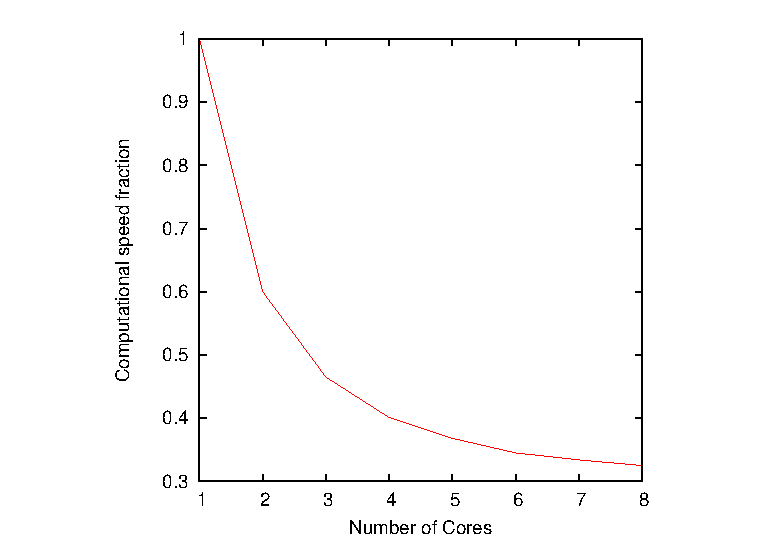
\includegraphics[scale=0.9]{corespeed.eps}
  \caption{Computation speed of simulations ran with different number of cores.
    The $y$-axis represents the fraction of time each core has in comparison to the the $1$-core result.
    Same simulation setup as the travelling wave simulation.
    Ran until $t = 2$ with a grid of $2049 \times 2049$. }
  \label{fig:corespeed}
\end{figure}

The implementation of Algorithm \ref{alg:iterateCM} was done with Fortran. 
The system is stored in diagonal format, since $A$ has five distinct diagonals.

All the computations were run on a custom built workstation with an Intel Xeon CPU E5-2650 (1.2 GHz, 20MB cache size) and 32 GB RAM under Red Hat Enterprise Linux Server release 6.5 (Santiago). 
Running the computations with OpenMP, took advantage of 4 out of the 16 threads of the Intel Xeon CPU, with 2 threads to each core.
The choice of 4 cores is because there is not enough computational gain from using extra, as shown in Figure \ref{fig:corespeed}.
The selection of 4 threads is because the computation time decrease becomes less efficient after more then 4 threads. 
The GNU Fortran compiler, version 4.4.7, was used for all computations; the compiler arguments were
\begin{verbatim} -03 -fdefault-real-8 -fopenmp \end{verbatim}



%!% Add other computers nd compilers to show that it was rigerously tested...

\section{Method Validation}

  With a defined method and computational setup we assess the behavior and accuracy of the method in a variety of simulations.
  An examination of a typical simulation will show if the expected behaviour is observed.
  A convergence analysis for the method can be done to confirm that solutions from different grid sizes approach a single solution as they become more precise.
  This convergence test will also show the thresholds for an accurate simulation result, to help reduce the computiation times.
  Once the fully-implicit method has been tested, it can be compared against the semi-implicit method.

\subsection{Basic Simulations}

  Using Algorithm \ref{alg:iterateCM}, simple scenarios can be tested as a first verification on the method.

  % Too simple/useless visual. Instead maybe have a graph of the standard deviation between gridpoints and show that it stays 0 (or constant?) with time.
  %
  %The most simple test would be homogenous initial conditions, $M = 0.1, C = 1 \forall x \in \Omega$.
  %This test would serve mainly as a confirmation that the method can solve (\ref{equ:model_system}) with the most trivial of initial conditions accurately.
  %The solutions in Figure \ref{fig:basic_homo} show that with homogenous initial conditions, the solution remains homogenous with time.
  %
  %\begin{figure}
  %  \centering
  %  \begin{tabular}{c}
  %  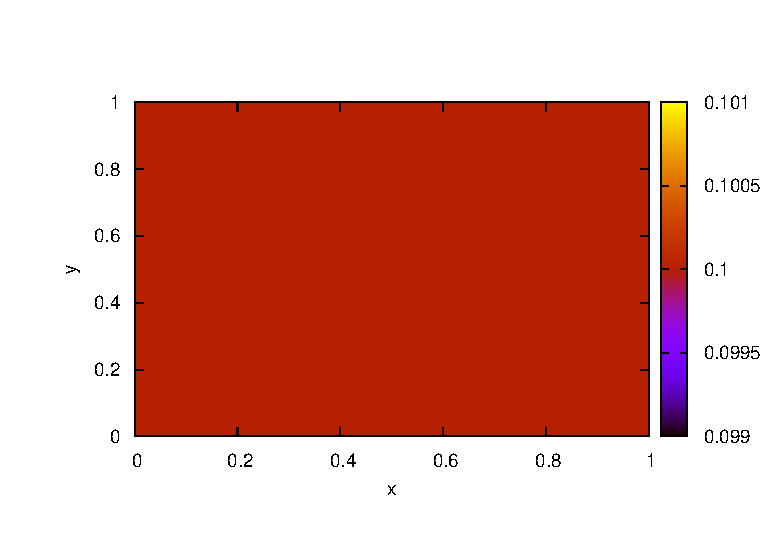
\includegraphics[scale = 0.8]{basic_homo_t0} \\ 
  %  (a) \\
  %  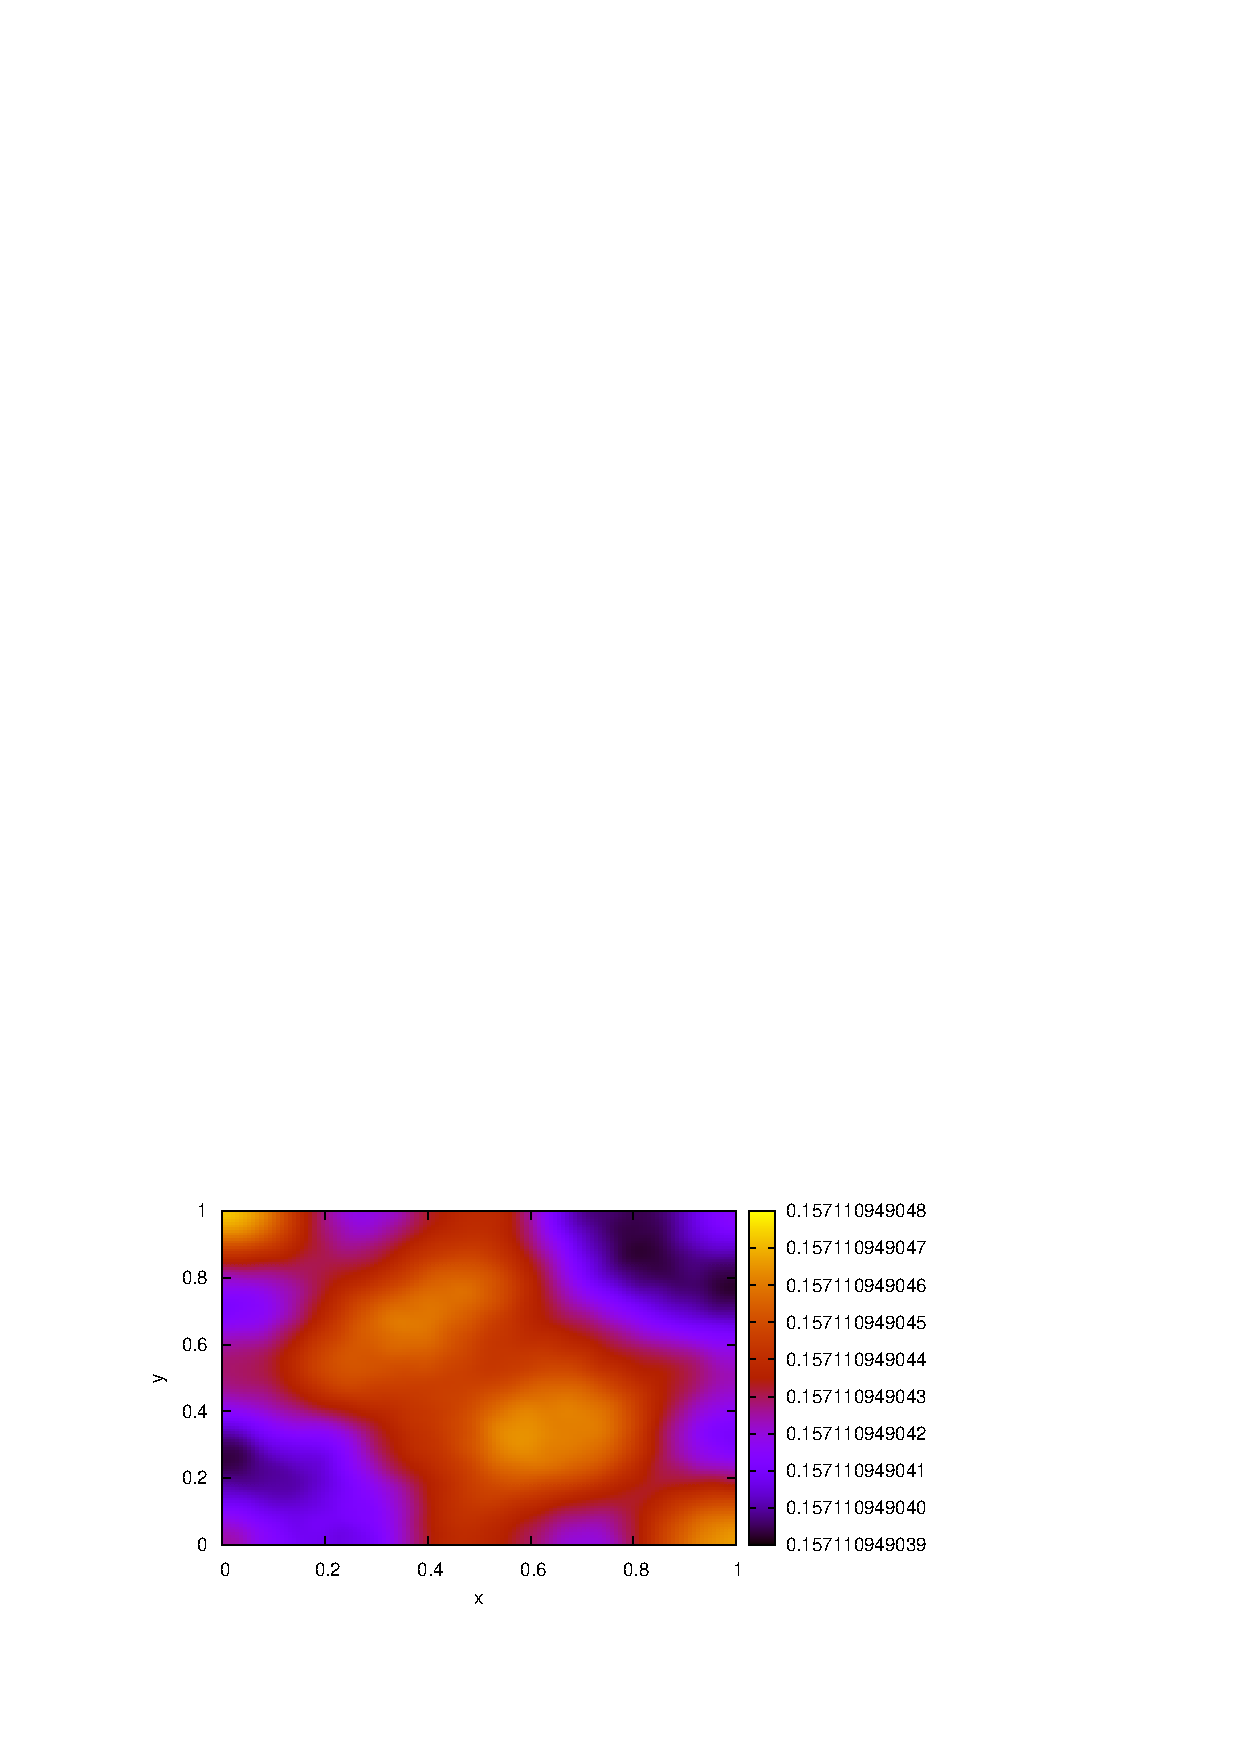
\includegraphics[scale = 0.8]{basic_homo_t10} \\
  %  (b)
  %  \end{tabular}
  %  \caption{Basic homogenous solutions, with $M = 0.1, C = 1 \forall x \in \Omega$. 
  %    The solution stay homogenous with time, as seen by comparing (a) the initial solution at $t = 0$, and (b) at $t = 10$.}
  %  \label{fig:basic_homo}
  %\end{figure}
  

  A simple test would be to check if the spatial discretization can preserve specific characteristics of the solutions.
  One example of this would be seeing if a 1D initial condition could be preserved as time progresses.
  Having all of the biomass on one boundary of $\Omega$, for example across the $y$-axis, would qualify as a 1D intial condition.
  These initial conditions will be defined as:
  \begin{equation} \label{equ:basic_init_trav_wave}
    \begin{aligned}
    M &= \begin{cases}
      -\left( \frac{h}{d^4} \right) x^4 + h & \text{, if } y \le d \\
      0 & \text{, otherwise}
    \end{cases} \\
    C &= 1
    \end{aligned}
  \end{equation}
  where $h = 0.1$ and $d = \frac{5}{128}$.
  Here, $h$ and $d$ represent the height and depth of the innoculation site. 

  The solution shown in Figure \ref{fig:basic_trav} shows that the 1D characteristic of the biomass stays at a later time. 

  \begin{figure}
    \centering
    \begin{tabular}{c c}
      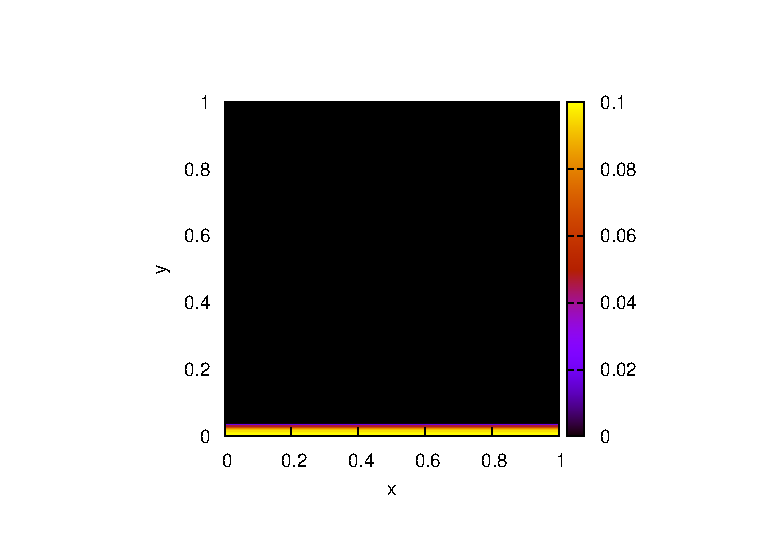
\includegraphics[scale = 0.7]{basic_trav_wave_M_t0} & 
      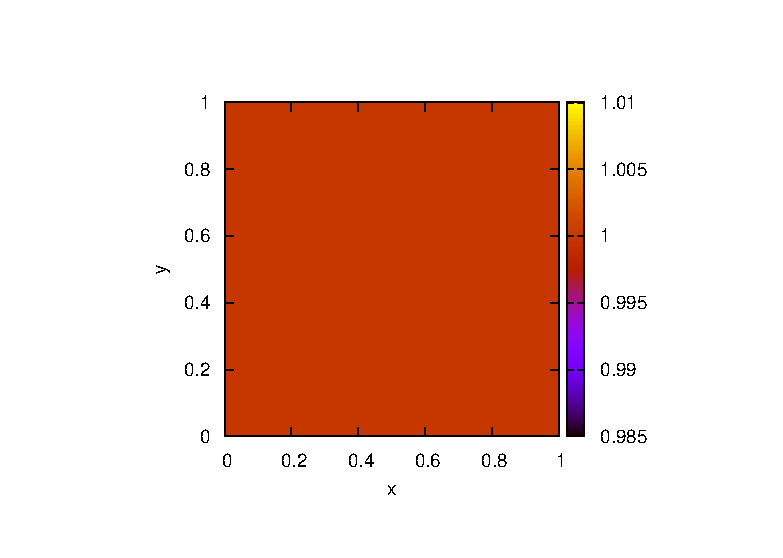
\includegraphics[scale = 0.7]{basic_trav_wave_C_t0} \\
      (a) & (b) \\
      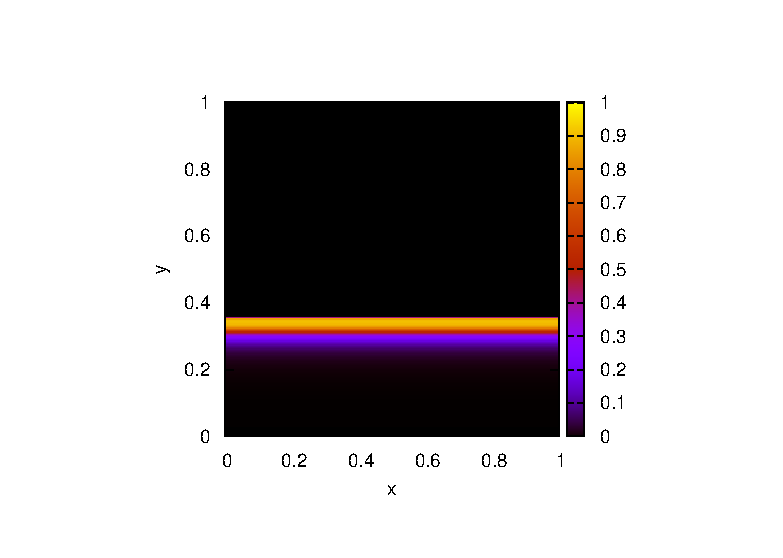
\includegraphics[scale = 0.7]{basic_trav_wave_M_t40} &
      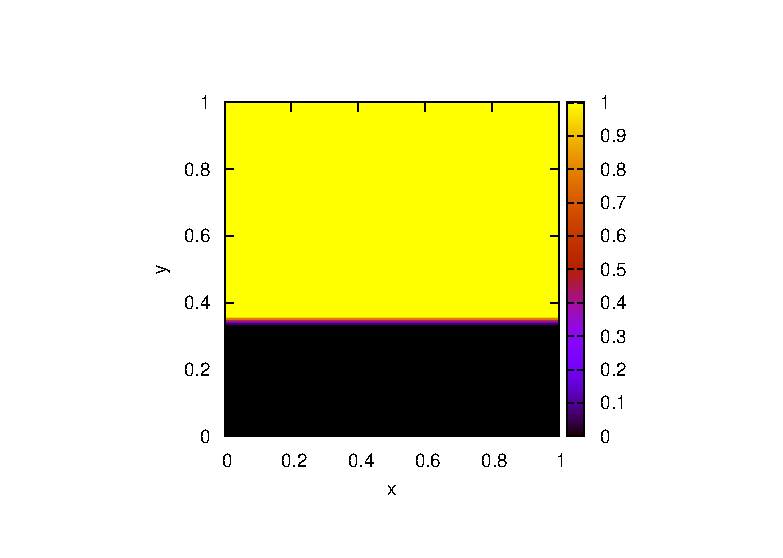
\includegraphics[scale = 0.7]{basic_trav_wave_C_t40}\\
      (c) & (d)
    \end{tabular}
    \caption{Solutions for (ac) $M$ and (bd) $C$ with 1D initial conditions defined in (\ref{equ:basic_init_trav_wave}) at (ab) $t = 0$ and (cd) $t = 40$. Computed with a $1025 \times 1025$ grid and a timestep of $\Delta t = 10^{-3}$.}
    \label{fig:basic_trav}
  \end{figure}

  Another characteristic to observe would be if a spherical initial condition remains spherical.
  Using intial conditions for the biomass,
  \begin{equation} \label{equ:basic_spherical}
    M = \begin{cases}
      - \frac{h}{d^2} \left( x - 0.5)^2 + (y - 0.5)^2 \right) + h  & \text{, if } (x - 0.5)^2 + (y - 0.5)^2 < d^2 \\
      0 & \text{, otherwise}
    \end{cases},
  \end{equation}
  a test can be tried to see if the spherical nature of the solution is kept as time progresses.
  The solution shown in Figure \ref{fig:basic_spherical} shows that the spherical shape of the solution is maintained at later times.

  \begin{figure}
    \centering
    \begin{tabular}{c c}
      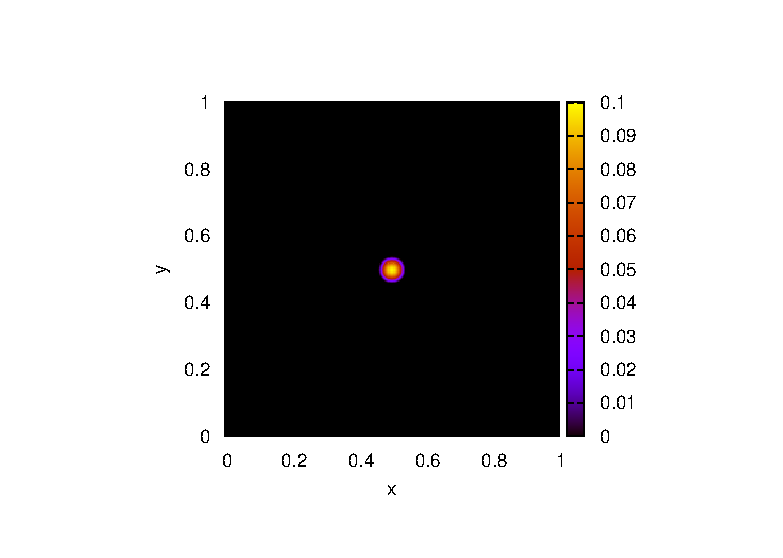
\includegraphics[scale = 0.7]{basic_spherical_M_t0} & 
      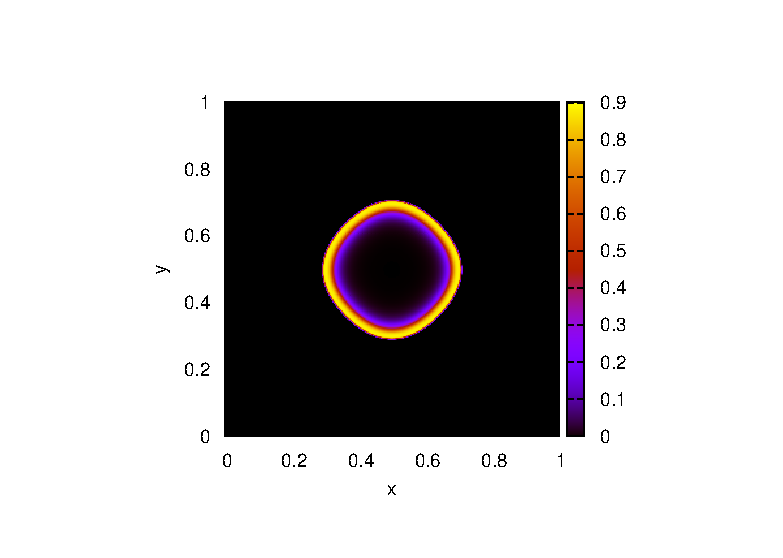
\includegraphics[scale = 0.7]{basic_spherical_M_t40} \\
      (a) & (b)
    \end{tabular}
    \caption{Solutions for $M$ with spherical initial conditions defined by (\ref{equ:basic_spherical}) at (a) $t = 0$ and (b) $t = 40$. Computed with a $1025 \times 1025$ grid and a timestep of $\Delta t = 10^{-3}$.}
    \label{fig:basic_spherical}
  \end{figure}
  
  Both Figure \ref{fig:basic_trav} and Figure \ref{fig:basic_spherical} increase the confidence that the spatial discretization did not introduce any loss of characteristics for the solutions.
    

  %!% Descibe the simulation that you carry out here in more detail, so the reader can follow.
  %!% Give the equations that I solve
 % \begin{equation}
 %   M_t = \nabla (D(M)\nable M) + aM
 % \end{equation}
 % also show the exct derivation (through the use of Divergence theorem and intergrating over \Omega with reference to the boundary conditions neumann) of:
 % \begin{equation}
 %   T_{M}(t) = T_M(0) e^{at}
 % \end{equation}
 % Also make FIG 3.4 a two-panel figure. One is the current plot and the other is the exact T_M and the numerical T_M, in logscaale.
 % Also should probably set the xr for the current plot so that it is only in the region of good numbers.
 % This time can be computed exactly, since I can a priori estimate from T_M(t), since I know that the maximum T_M can be is the total value of Omega??(namely M=1 everywhere)

  Given the boundary conditions and spatial discretization, there could be a possible source or sink of biomass when it must diffuse along the boundary of the region.
  To ensure this is not the case, the total amount of biomass can be used to compare the simulated amount against the theoretical amount. 
  However, the total biomass cannot be exactly determined with the given growth rate function.
  This means that there will not be anything to measure the validity of the simulation solution against.
  If we let the growth rate be some constant called $a$, the exact total biomass can be calculated.

  The expected total biomass would be of the form $y_0 e^{at}$.
  This can be checked by tracking the total biomass, now called $T_{M}(t)$, with the changed growth rate function, $F(C) = a$.
  The calculation of $T_{M}(t)$ can be done by,
  \begin{equation} \label{equ:total_biomass}
    T_{M}(t) = \int_{\Omega} M(t) dx.
  \end{equation}
  Numerically, this is computed by grid-wise summation,
  \begin{equation}
    T_{M}(t^k) \approx T_{M}^{k} = \frac{ \sum^n_i \sum^m_j M^{k}_{i,j} }{nm}.
  \end{equation}

  The simulation setup used will be analogous to that used for Figure \ref{fig:basic_spherical}.
  The one difference will be that the simulation here is ran for a longer time to allow the biomass to diffuse along the boundary, showing the boundary effects.
 
  From Figure \ref{fig:basic_growth} we can see that the total biomass only differs between the computed value and the theoretical value by a relative error less then $0.003$.
  The cases where the error becomes significant are from the region being completely filled with biomass, at which point diffusion is no longer possible.
  The error fluctuates violently here because of this.
  This suggests that the method does not introduce any significant sources or sinks of biomass at the boundary of the region.

  \begin{figure}
    \centering
    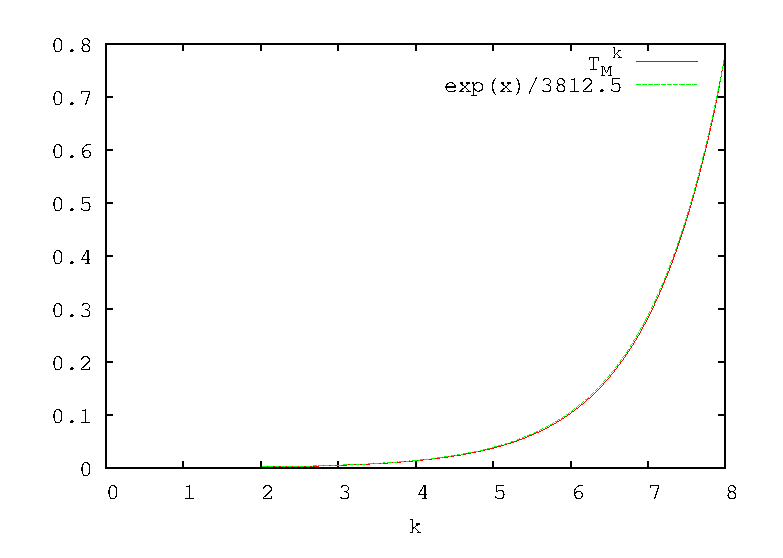
\includegraphics[scale = 0.9]{basic_growth}
    \caption{Plot of the relative error, $\frac{|f_1 - f_2|}{|f_2|}$, between the computed total biomass, $f_1 = T_{M}(t)$, and the theoretical total biomass, $f_2 = y_0 e^x$. 
      The changes after $t = 8$ are from the biomass having completely filled the region $\Omega$.
      This means that there is no physical space for the biomass to occupy and thus the growth slows down to a stop.}
    \label{fig:basic_growth}
  \end{figure}
  
  %!% add mass -conseration between M and C by checking that $M' + \gamma C' = 0$; ie total mass is constant
    % Show here the pre-work of integrating over the domain and that the spatial term dissapers and all thats left is the growth terms in both M and C.
    % If its interesting, show a graph of M'+gama C vs. t, and try to explain/justify the changes it makes (unless its 0, then just report that its zero and say DATA NOT SHOWN.

\subsection{Convergence Analysis}
  %!%To validate the accuracy of the method, convergence analyses on the spatial and temporal discretizations will need to be made. 
  To validate the accuracy of the method, convergence analyses on the spatial discretizations will need to be made. 
  Then the comparison between the semi- and fully-implicit method established in Algorithm \ref{alg:iterateCM} can investigated.
  First, a metric must be formed to enable consistent comparisons between different simulation solutions. 
  This metric will be referred to as the normed difference. 
  Only $M$ will be considered for the normed difference calculations.
  This is because $C$ depends on $M$ and including it does not qualitativly change the results.

\subsubsection{Normed Difference Computations}

  The normed difference is computed by taking the relative normed-difference between two solution in the following fashion:
  \begin{equation} \label{equ:normed difference_comp}
    \epsilon_{sol} = \frac{||u_1 - u_2||}{||u_2||}
  \end{equation}
  where $u_1$ represents one simulation solution and $u_2$ represents the solution that is theoretically more accurate.
  The theoretical accuracy of $u_2$ derives from the fact that most comparisons will be done between solutions where one is trivially expected to be more precise.
  For our purposes, the solutions we compare will typically vary in only $\Delta x$ or between semi- and fully- implicit.
  These are understood to have the relation that a smaller $\Delta x$, and that the fully-implicit method with the highest tolerance is to be more accurate.
  There is an assumption that both $u_1$ and $u_2$ have the same number of grid points, so that the difference can be taken grid-wise.

  The results of the normed difference computations, named $\epsilon_{sol}$, is a numerical value for the difference between two solutions.
  This depends on the norm used during the computations.
  Here three norms will be used:
  \begin{equation}  \label{equ:norm_l1}
    \ell_1: ||u||_1 = \frac{1}{nm} \sum_{i}^{nm} |u_{i}|
  \end{equation}
  \begin{equation}  \label{equ:norm_l2}
    \ell_2: ||u||_2 = \frac{1}{nm} \sqrt{\sum_{i}^{nm} (u_{i})^2}
  \end{equation}
  \begin{equation}  \label{equ:norm_linf}
    \ell_\infty: ||u||_\infty = \max_{i=1,\ldots,nm} |u_{i}|
  \end{equation}
  These different norms will all be used to create a broader understanding of the normed difference.
  This creates three distinct values for $\epsilon_{sol}$, named $\epsilon_{\ell_1}$, $\epsilon_{\ell_2}$, and $\epsilon_{\ell_\infty}$; each named for the norm used during the computation.
  Note that these norms are for the vector for of the solution, throught the use of the grid-ordering $\pi(i,j)$.
  
 %!% \item What program did I use? (R probably....)
 %!% \item Maybe run though a trivial Fisher equation problem to confirm that it works ?
  % Also mention the Accuracy of the solutions by using the norm of each solution compared to the  most accurate one.... (Maybe take a solution at a higher grid resolution?, not sure what to do here)

\subsubsection{Grid Size Convergence}
  To observe the validity of the method, a test on the convergence of solutions based on the spatial discritization is done.
  This will involve using the same simulation described in (\ref{equ:basic_init_trav_wave}) due to the simplicity. 
 
  The convergence will be tracked with only two forms of $\epsilon_{sol}$; $\epsilon_1$ and $\epsilon_2$.
  %!% Might as well include the values of \epsilon_infty in with the results and discuss why it isn't a good measure in the cases where it blatently looks bad.
  This is because the value of $\epsilon_{\infty}$ doesn't vary with the grid size, since the wave front has a steep interface and tends to lead to inconsistent changes in normed difference.
  Since the use of $\epsilon_{\infty}$ is not a suitable method for measuring the normed difference, the inconsistency does not suggest an invalidity with the method.
  Because of the difference in the number of grid points between different solutions, $u_1$ and $u_2$, only the grid points in the coarser refinement will be used.
  This places a limitation on the selection of grid-sizes since there must be some grid points locations that are the same for two different chosen grid sizes.
  For this purpose, we define the function $s(n) = 2^{n}+1$ for $n \in \mathbb{N}$ to be used as the grid size selection function.
  Now certain grid points will match without the use of linear interpolation, as illustrated in Figure \ref{fig:grid_point_lineup}.
 % Here we do not use the typical grid doubling, $2^n$, because no grid points equal between two different grid size selection, as illustrated in Figure \ref{fig:grid_point_lineup}.


  \begin{figure}
    \centering
    \begin{tabular}{| c | c |}
      \hline
      &  $s(n) = 2^{n}+1 $ \\
      \hline
      $n=2$ 
      & 
      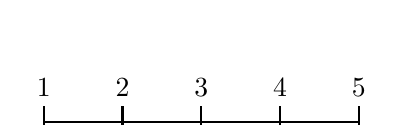
\begin{tikzpicture}
        \draw [thick] (0.0, 1.0) -- (4.0, 1.0);
        \draw [thick] (0.0, 0.8) -- (0.0, 1.2);
        \draw [thick] (1.0, 0.8) -- (1.0, 1.2);
        \draw [thick] (2.0, 0.8) -- (2.0, 1.2);
        \draw [thick] (3.0, 0.8) -- (3.0, 1.2);
        \draw [thick] (4.0, 0.8) -- (4.0, 1.2);

        \node [above] at (0.0, 1.2) {1};
        \node [above] at (1.0, 1.2) {2};
        \node [above] at (2.0, 1.2) {3};
        \node [above] at (3.0, 1.2) {4};
        \node [above] at (4.0, 1.2) {5};
      \end{tikzpicture} 
      \\
      \hline
      $ n = 3 $
      &
      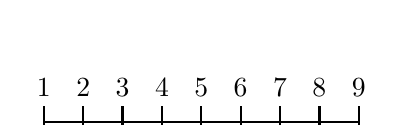
\begin{tikzpicture}
        \draw [thick] (0,1) -- (4,1);
        \draw [thick] (0.0, 0.8) -- (0.0, 1.2);
        \draw [thick] (0.5, 0.8) -- (0.5, 1.2);
        \draw [thick] (1.0, 0.8) -- (1.0, 1.2);
        \draw [thick] (1.5, 0.8) -- (1.5, 1.2);
        \draw [thick] (2.0, 0.8) -- (2.0, 1.2);
        \draw [thick] (2.5, 0.8) -- (2.5, 1.2);
        \draw [thick] (3.0, 0.8) -- (3.0, 1.2);
        \draw [thick] (3.5, 0.8) -- (3.5, 1.2);
        \draw [thick] (4.0, 0.8) -- (4.0, 1.2);

        \node [above] at (0.0, 1.2) {1};
        \node [above] at (0.5, 1.2) {2};
        \node [above] at (1.0, 1.2) {3};
        \node [above] at (1.5, 1.2) {4};
        \node [above] at (2.0, 1.2) {5};
        \node [above] at (2.5, 1.2) {6};
        \node [above] at (3.0, 1.2) {7};
        \node [above] at (3.5, 1.2) {8};
        \node [above] at (4.0, 1.2) {9};
      \end{tikzpicture}
      \\
      \hline
    \end{tabular}
    \caption{Visualization in 1D to illustrate the choice of $s(n) = 2^{n} + 1 $ instead of $2^{n}$ for the grid size selection.
      Here is can be seen that successive grid size selections using $s(n)$ line up on certain grid points and when using $2^n$ no grid points are equivalent.}
    \label{fig:grid_point_lineup}
  \end{figure}

  %!% This figure has the 2^n lineup also
  %\begin{figure}
    % \centering
    % \begin{tabular}{| c | c | c |}
    %   \hline
    %   &  $s(n) = 2^{n}+1 $ & $2^n$ \\
    %   \hline
    %   $n=2$ 
    %   & 
    %   \begin{tikzpicture}
    %     \draw [thick] (0.0, 1.0) -- (4.0, 1.0);
    %     \draw [thick] (0.0, 0.8) -- (0.0, 1.2);
    %     \draw [thick] (1.0, 0.8) -- (1.0, 1.2);
    %     \draw [thick] (2.0, 0.8) -- (2.0, 1.2);
    %     \draw [thick] (3.0, 0.8) -- (3.0, 1.2);
    %     \draw [thick] (4.0, 0.8) -- (4.0, 1.2);

    %     \node [above] at (0.0, 1.2) {1};
    %     \node [above] at (1.0, 1.2) {2};
    %     \node [above] at (2.0, 1.2) {3};
    %     \node [above] at (3.0, 1.2) {4};
    %     \node [above] at (4.0, 1.2) {5};
    %   \end{tikzpicture} 
    %   &
    %   \begin{tikzpicture}
    %     \draw [thick] (0,1) -- (4,1);
    %     \draw [thick] (0.0, 0.8) -- (0.0, 1.2);
    %     \draw [thick] (1.333, 0.8) -- (1.333, 1.2);
    %     \draw [thick] (2.667, 0.8) -- (2.667, 1.2);
    %     \draw [thick] (4.0, 0.8) -- (4.0, 1.2);

    %     \node [above] at (0.0, 1.2) {1};
    %     \node [above] at (1.333, 1.2) {2};
    %     \node [above] at (2.667, 1.2) {3};
    %     \node [above] at (4.0, 1.2) {4};
    %   \end{tikzpicture}
    %   \\
    %   \hline
    %   $ n = 3 $
    %   &
    %   \begin{tikzpicture}
    %     \draw [thick] (0,1) -- (4,1);
    %     \draw [thick] (0.0, 0.8) -- (0.0, 1.2);
    %     \draw [thick] (0.5, 0.8) -- (0.5, 1.2);
    %     \draw [thick] (1.0, 0.8) -- (1.0, 1.2);
    %     \draw [thick] (1.5, 0.8) -- (1.5, 1.2);
    %     \draw [thick] (2.0, 0.8) -- (2.0, 1.2);
    %     \draw [thick] (2.5, 0.8) -- (2.5, 1.2);
    %     \draw [thick] (3.0, 0.8) -- (3.0, 1.2);
    %     \draw [thick] (3.5, 0.8) -- (3.5, 1.2);
    %     \draw [thick] (4.0, 0.8) -- (4.0, 1.2);

    %     \node [above] at (0.0, 1.2) {1};
    %     \node [above] at (0.5, 1.2) {2};
    %     \node [above] at (1.0, 1.2) {3};
    %     \node [above] at (1.5, 1.2) {4};
    %     \node [above] at (2.0, 1.2) {5};
    %     \node [above] at (2.5, 1.2) {6};
    %     \node [above] at (3.0, 1.2) {7};
    %     \node [above] at (3.5, 1.2) {8};
    %     \node [above] at (4.0, 1.2) {9};
    %   \end{tikzpicture}
    %   &
    %   \begin{tikzpicture}
    %     \draw [thick] (0,1) -- (4,1);
    %     \draw [thick] (0.000, 0.8) -- (0.000, 1.2);
    %     \draw [thick] (0.571, 0.8) -- (0.571, 1.2);
    %     \draw [thick] (1.143, 0.8) -- (1.143, 1.2);
    %     \draw [thick] (1.714, 0.8) -- (1.714, 1.2);
    %     \draw [thick] (2.286, 0.8) -- (2.286, 1.2);
    %     \draw [thick] (2.857, 0.8) -- (2.857, 1.2);
    %     \draw [thick] (3.429, 0.8) -- (3.429, 1.2);
    %     \draw [thick] (4.000, 0.8) -- (4.000, 1.2);

    %     \node [above] at (0.000, 1.2) {1}; 
    %     \node [above] at (0.571, 1.2) {2};
    %     \node [above] at (1.143, 1.2) {3};
    %     \node [above] at (1.714, 1.2) {4};
    %     \node [above] at (2.286, 1.2) {5};
    %     \node [above] at (2.857, 1.2) {6};
    %     \node [above] at (3.429, 1.2) {7};
    %     \node [above] at (4.000, 1.2) {8};

    %   \end{tikzpicture}
    %   \\
    %   \hline
    % \end{tabular}
    % \caption{Visualization in 1D to illustrate the choice of $s(n) = 2^{n} + 1 $ instead of $2^{n}$ for the grid size selection.
    %   Here is can be seen that successive grid size selections using $s(n)$ line up on certain grid points and when using $2^n$ no grid points are equivalent.}
    % \label{fig:grid_point_lineup}
  %\end{figure}

  
  %!% Makes this use log graph and maybe its a stragith line.
  %!% Also have graphs of how the quatilites of interest change with grid-size (and with t?)
  %!% Maybe have a 2D plot of x = \delta x, y = \delta t, z = \epsilon. showing how it (should) decrease with \delta x and \t.
  %     to the above graph, can later add computation time to it to justify the choice in \delta t and \delta x for the later simulations

  Using the same simulation setup as was done in Figure (\ref{fig:basic_trav}), solutions resulting from different grid sizes based on $s(n)$ are computed for $n = 5, 6, \ldots, 12$.
  In this case, when calculating $\epsilon_{sol} = \frac{| u_1 - u_2 |}{|u_2|}$, we let $u_1$ be the grid size under investigation and $u_2$ be the solutions of the most refined gridsize, $n = 12$.
  This would show the converging solutions for smaller grid sizes because the change to the finest grid size will be monotonically decreasing.

  \begin{figure}
    \centering
    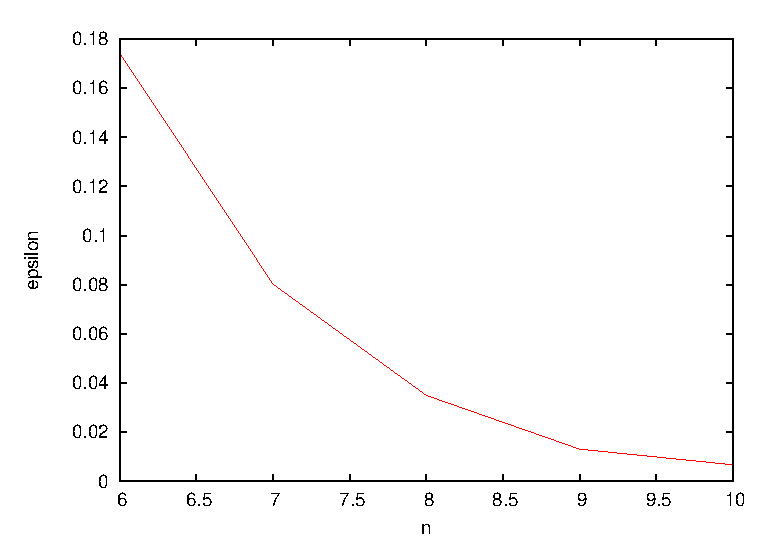
\includegraphics{converge_spatial}
    %!% State here the final t for which these calculations were made.
    \caption{Plot showing the convergence of solutions based on changes in $\Delta x$. The computions are of $\epsilon_{\ell_1}$ and $\epsilon_{\ell_2}$ with grid-size following $s(n) = 2^{n}+1$.}
    \label{fig:converge_spatial}
  \end{figure}
  %!% Describe that the hickup at n=6 is because n=5 is too coarse to fit with the initial condition
  %!% to add to this: include a 4-8 panel time evolution with the differernt gridsizes superimposed at each panel. i.e (a) is t=0, so have n=5...12 all plotted at t=0 in graph (a). Do the same for (b) t = 10 (for example) (c) t = 20 etc.... This will show how the gridsizes do/don't change the actual visual of the solution
  %!% To do the above: use the trav-wave IC and 1D visualization. Simply state that we will take for granted a priori that the 2D region can be reduced to 1D.
  %!% Also state out here the final t for which the normed difference calculations were made.

  The results from Figure \ref{fig:converge_spatial} show that the solutions converge as the grid size become refined with the grid size.
  The nonmonotonicity for $n = 5$ is because the grid has become too large for predictable calculations, which is an acceptible error since such a coarse grid would never be used for computational simulations.

%!% Also, check the results with a larger and smaller $\Delta t$ to see if they change.

%\subsubsection{$\Delta t$ Convergence}
%
%  A similar convergence analysis will also be performed for the temporal discritizations.
%  This is simply to confirm that the selection of $\Delta t$ is optimal for computation time and for accuracy.
%  The 
%
%  \begin{figure}
%    \centering
%    \begin{tabular}{c c}
%%    \includegraphics{converge_temporal_a.eps} &
%%    \includegraphics{converge_temporal_a.eps} \\
%    (a) & (b) \\
%%    \includegraphics{converge_temporal_a.eps} &
%%    \includegraphics{converge_temporal_a.eps} \\
%    (c) & (d)
%    \end{tabular}
%    \caption{A series of plots showing the convergece of solutions based on changes in $\Delta t$ using $eSoln = 10^n$ for (a) $n = -1$, (b) $n = -4$, (c) $n = -8$, and (d) $n = -12$.} 
%
%  \end{figure}
 
%\subsection{Table of Results}
%
%That list, compute time, "normed difference", number of iterations of linear solver, and number of iterations for ALgorithm 1 for a series of $\epsilon_{sol}$.
%Do this table for a larger $\Delta t$ to see if the algorithm allows for a faster computation with the larger timesteps.
%
%Be extrodinaryly pedantic on everything here.
%Try for something like a paragraph for each item in the table; explain how it's computed, why we pick this measure, what we expect, and what it will say about the results....
%



\pagestyle{chp3-5} % Since the chapter name is too long for the header.
\section{Comparison of Semi-implicit and Fully-implicit Method}
  Here the main comparison that analyses the effects of using Algorithm \ref{alg:iterateCM} with different tolerances. 
  Recall that the main observation is for $tol. = 1$, which correlates to the semi-implicit method since it will allow only a single iteration of the algorithm. 

  The simulation used is the same as described in (\ref{fig:basic_trav}).
  The comparison will be on multiple metrics: the average number of iterations of Algorithm \ref{alg:iterateCM}, the value of $\epsilon_1$ and $\epsilon_2$, the computation time of the simulation, and the location of the wave peak.

  The average number of iterations are tracked so that an idea of the extra work can be formed.
  As the tolerance decreases the amount of iterations the algorithm must perform will increase, the degree of increase will help relate the amount of work.

  The value of $\epsilon_1$ and $\epsilon_2$ act as a measure of accuracy.
  Here, these values correspond to the difference between a pair of solutions, $u_1$ and $u_2$.
  The $(u_1, u_2)$ pairs are: $(1, 10^{-8}), (10^{-8}, 10^{-10}), (10^{-10}, 10^{-12}), (10^{-12}, 10^{14})$.
  Each row of Table \ref{tab:tolerance_comparison} refers to the $u_1$ values of the pairs.
  Each difference was taken at the last timestep.

  Along with accuracy, the simulation time is tracked.
  This is because it represents another metric for which the viability of the fully-implicit method can be verified.
  Theoretically there should be a decrease in the error with the fully-implicit method as the value for $tol$ decreases.
  Therefore, this needs to be weighted against the cost of computational intensity and the increase of the simulation time.

  The location of the wave peak is a tracked quality of the solution that reveals how consistent the results are.
  The wave peak is described here as the maximum value of the solution at the final timestep calculated.
  The ultimate goal is that the simulation solutions be converging towards the exact solution.
  To see this here the $x$-coordinate of the wave peak is tracked.

  The results of the method comparison can be seen in Table \ref{tab:tolerance_comparison}.
  \begin{table}[h!tb]
  \centering
  \begin{tabular}{|c|c|c|c|c|c|}
    \hline
    Tol. & Avg. Iter. & $\epsilon_1$ & $\epsilon_2$ & Time & Wave Peak \\
    \hline
    $10^{-0}$  & 1.000 & 3.3501735409237e-08 & 8.4737222488052e-09 & 12.307 & 0.46484375\\
    $10^{-8}$  & 2.585 & 2.3362854691984e-04 & 1.0693478663953e-03 & 17.421 & 0.4609375\\
    $10^{-10}$ & 3.222 & 1.4801513256808e-05 & 1.0209699060817e-05 & 18.967 & 0.4609375\\
    $10^{-12}$ & 36.31 & 1.9170550231906e-04 & 1.3049331099727e-04 & 106.002 & 0.4609375\\
    \hline
  \end{tabular}
  \caption{Results from running simulations with different Tol.}
  \label{tab:tolerance_comparison}
\end{table}


  %!% Talk about what is seen here?

  %!% The fully-implicit method should have less iterations of the linear solver.
  
  %\begin{table}[h!tb]
  %  \centering
  %  %!% If I just list time and epsilons, maybe four gnuplots graph with the simulation time listed in the legend would be better.
  %  \begin{tabular}{|c|c|c|c|c|}
  %    \hline
  %    P & Simulation Time & $\epsilon_{\ell_1}$ & $\epsilon_{\ell_2}$ & $\epsilon_{\ell_\infty}$  \\
  %    \hline
  %    1& 60.05 & 0.0018 & - & - \\
  %    2& 97.72  & 0.0014 & - & - \\
  %    3& 117.46 & 0.0013 & - & - \\
  %    4& 126.44 & 0.0011& - & - \\
  %    \hline
  %    %!% OLD ROWS - Tol. 1 & Computation Time & $\epsilon_{sol}$ & Avg. Iter. 1 & Max Iter. 1 & Avg. Iter. 2 & Max Iter. 2 \\
  %  \end{tabular}
  %  \caption{Results from running simulation with different $P$ values. Note, $P = 1$ corresponds to the semi-implicit method.}
  %  \label{tab:tolerance_comparison}
  %\end{table}
  

\chapter{Simulation Results}
\pagestyle{normal}
\section{Typical Simulation}

A typical simulation refers to the parameter values and the choice of initial condition.
It will show the behaviour of the system under normal circumstances and help reveal interesting characteristics.

The typical initial condition attempts to emulate the biological situation of biomass growing inwards on a sheet of cellulose.
This will show how the biomass moves and how two separate masses interact when merging.
The initial condition used will initialize a number of random spherical inoculation points near the $y=0$ and $y=1$ axis.
We let $(x_r, y_r)$ be the random point used as the center for inoculation.
To separate the inoculation points we have $x_r \in [0,1]$ and $y_r \in [0, 0.1] \cup [0.9, 1]$.
The number of inoculation points are the same for both the $y=0$ region and $y=1$ region.
Multiple inoculation points combine additively.
Each spherical inoculation point is computed as,
\begin{equation} \label{equ:typical_initial_cond}
  M(0,x,y) = \frac{-h}{d^2} \left( (x-x_r)^2 + (y - y_r)^2 \right) + h, \quad M \ge 0.
\end{equation}
Note that $M(0,x,y)$ is for points within circles of radius $d$ centered at $(x_r, y_r)$, otherwise $M(0,x,y) = 0$.
For the substratum we have $C(0,x,y) = 1$ everywhere.

The choice of parameter value is based on the default values given in Table \ref{tab:default-parameters}.
There are $40$ inoculation points on each side, totalling $80$.
The fully-implicit method is used here with $tol = 10^{-8}$.

\subsection{Biomass Ratio}

\begin{figure}[!htp]
  \centering
  \begin{tabular}{c c}
      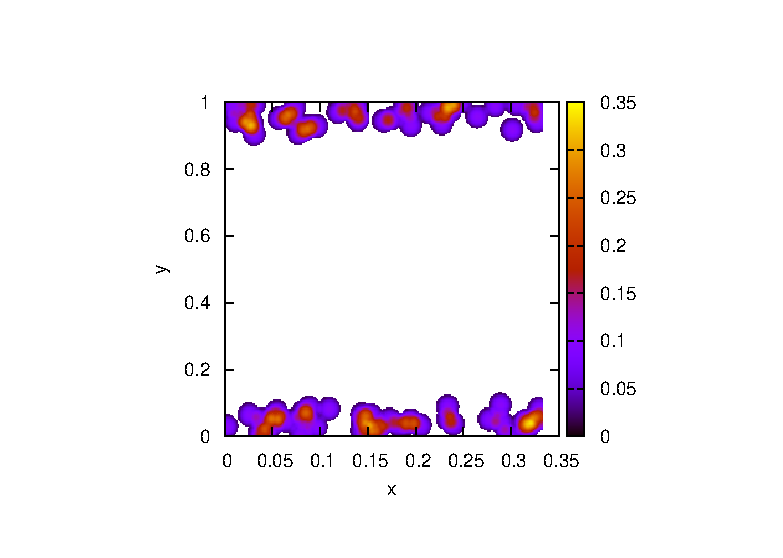
\includegraphics[scale=0.55]{typical_t0.eps} &
      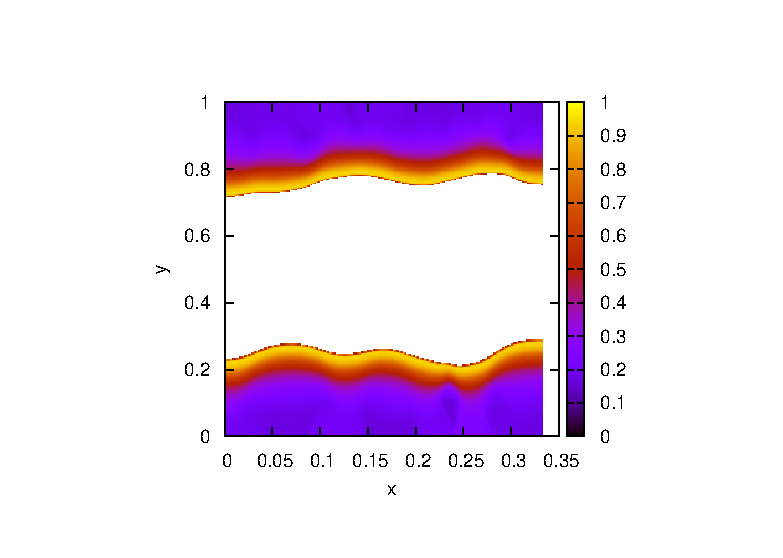
\includegraphics[scale=0.55]{typical_t2.eps} \\
      $t = 0$ & $t = 2$ \\
      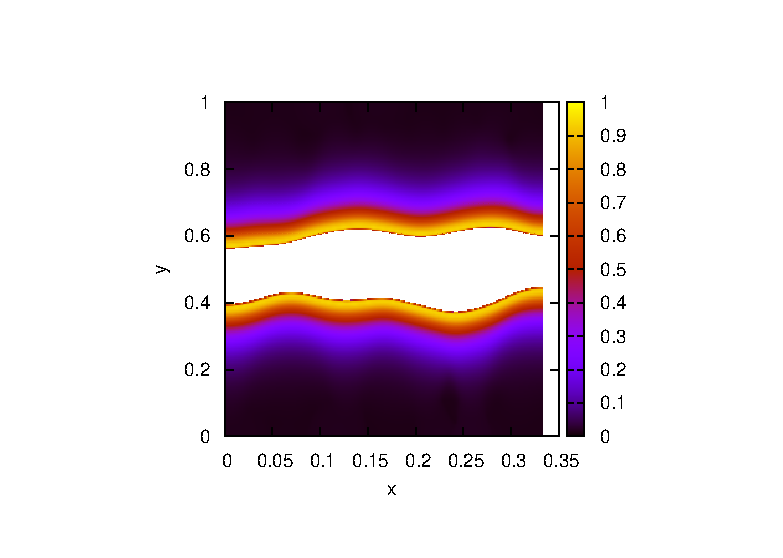
\includegraphics[scale=0.55]{typical_t3_67.eps} &
      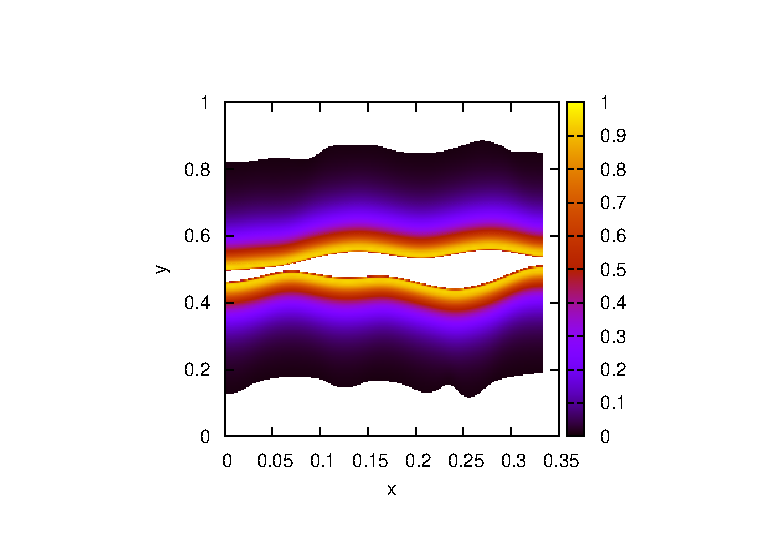
\includegraphics[scale=0.55]{typical_t5_33.eps} \\
      $t = 3.67$ & $t = 5.33$ \\
      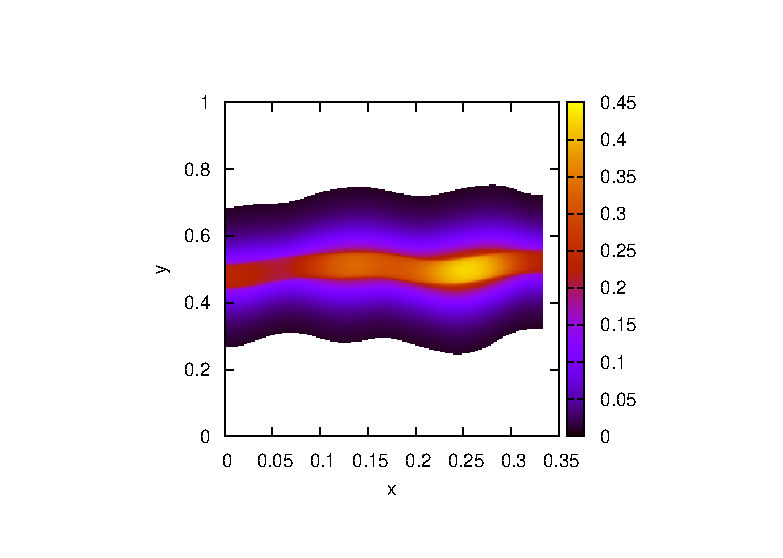
\includegraphics[scale=0.55]{typical_t7.eps} &
      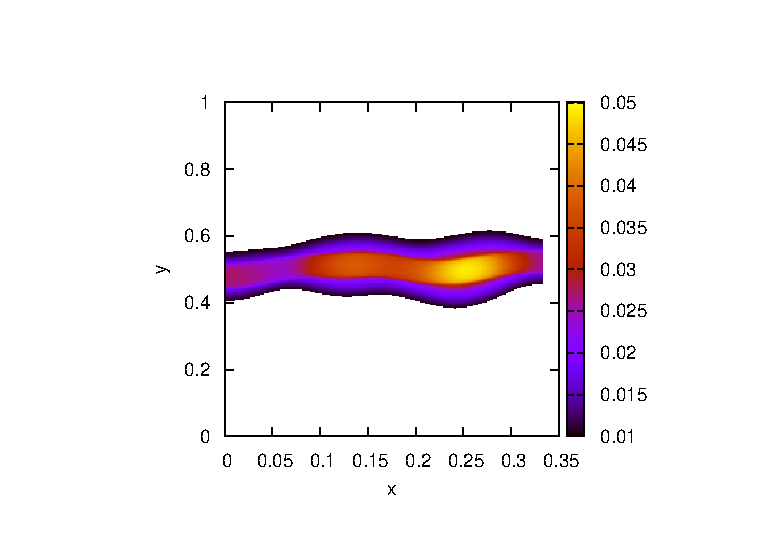
\includegraphics[scale=0.55]{typical_t9.eps} \\
      $t = 7$ & $t = 9$
   \end{tabular}
  \caption{A graph showing the $M$ solution of a typical simulation at different time steps.
    The initial condition is $80$ random spherical inoculation points evenly divided between each of the $y=0$ and $y=1$ sides.
    A $513 \times 513$ grid was used.  }
  \label{fig:typical_sim}
\end{figure}

Figure \ref{fig:typical_sim} shows the time evolution of $M$ for the simulation.
Here, the random inoculations on both sides of the region propagate towards each other and eventually combine at the center.
By looking at $t=2$, $t=3.67$, and $t = 5.33$ it appears as though the wave front is moving with a constant shape and at a constant speed.
This suggest that there may be the existence of a travelling wave solution which will be explored in the next section.

One important feature to notice is that the time evolution in Figure \ref{fig:typical_sim} matches the conceptual model proposed in \cite{dumitrache2015mathematicalModeling}.
This model can be seen in Figure \ref{fig:alex_schema}.
The different stages of the conceptual model can be observed in our simulation results: 
\begin{itemize}
  \item Stage I: $t = 2$ and $t = 3.67$ show the biomass growing towards the center of the sheet, which is the center white area.
  \item Stage II/III: $t = 5.33$ shows the consumed substrate region as the outer white.
  \item Stage IV: Not shown. Only occurs at the moment when the two bands first collide and the biomass concentration at that point still remains at the actual carrying capacity.
  \item Stage V: $t = 7$ and $t = 9$ show the combined center band, now at a biomass concentration lower then the actual carrying capacity.
\end{itemize}

\begin{figure}[!htp]
  \centering
  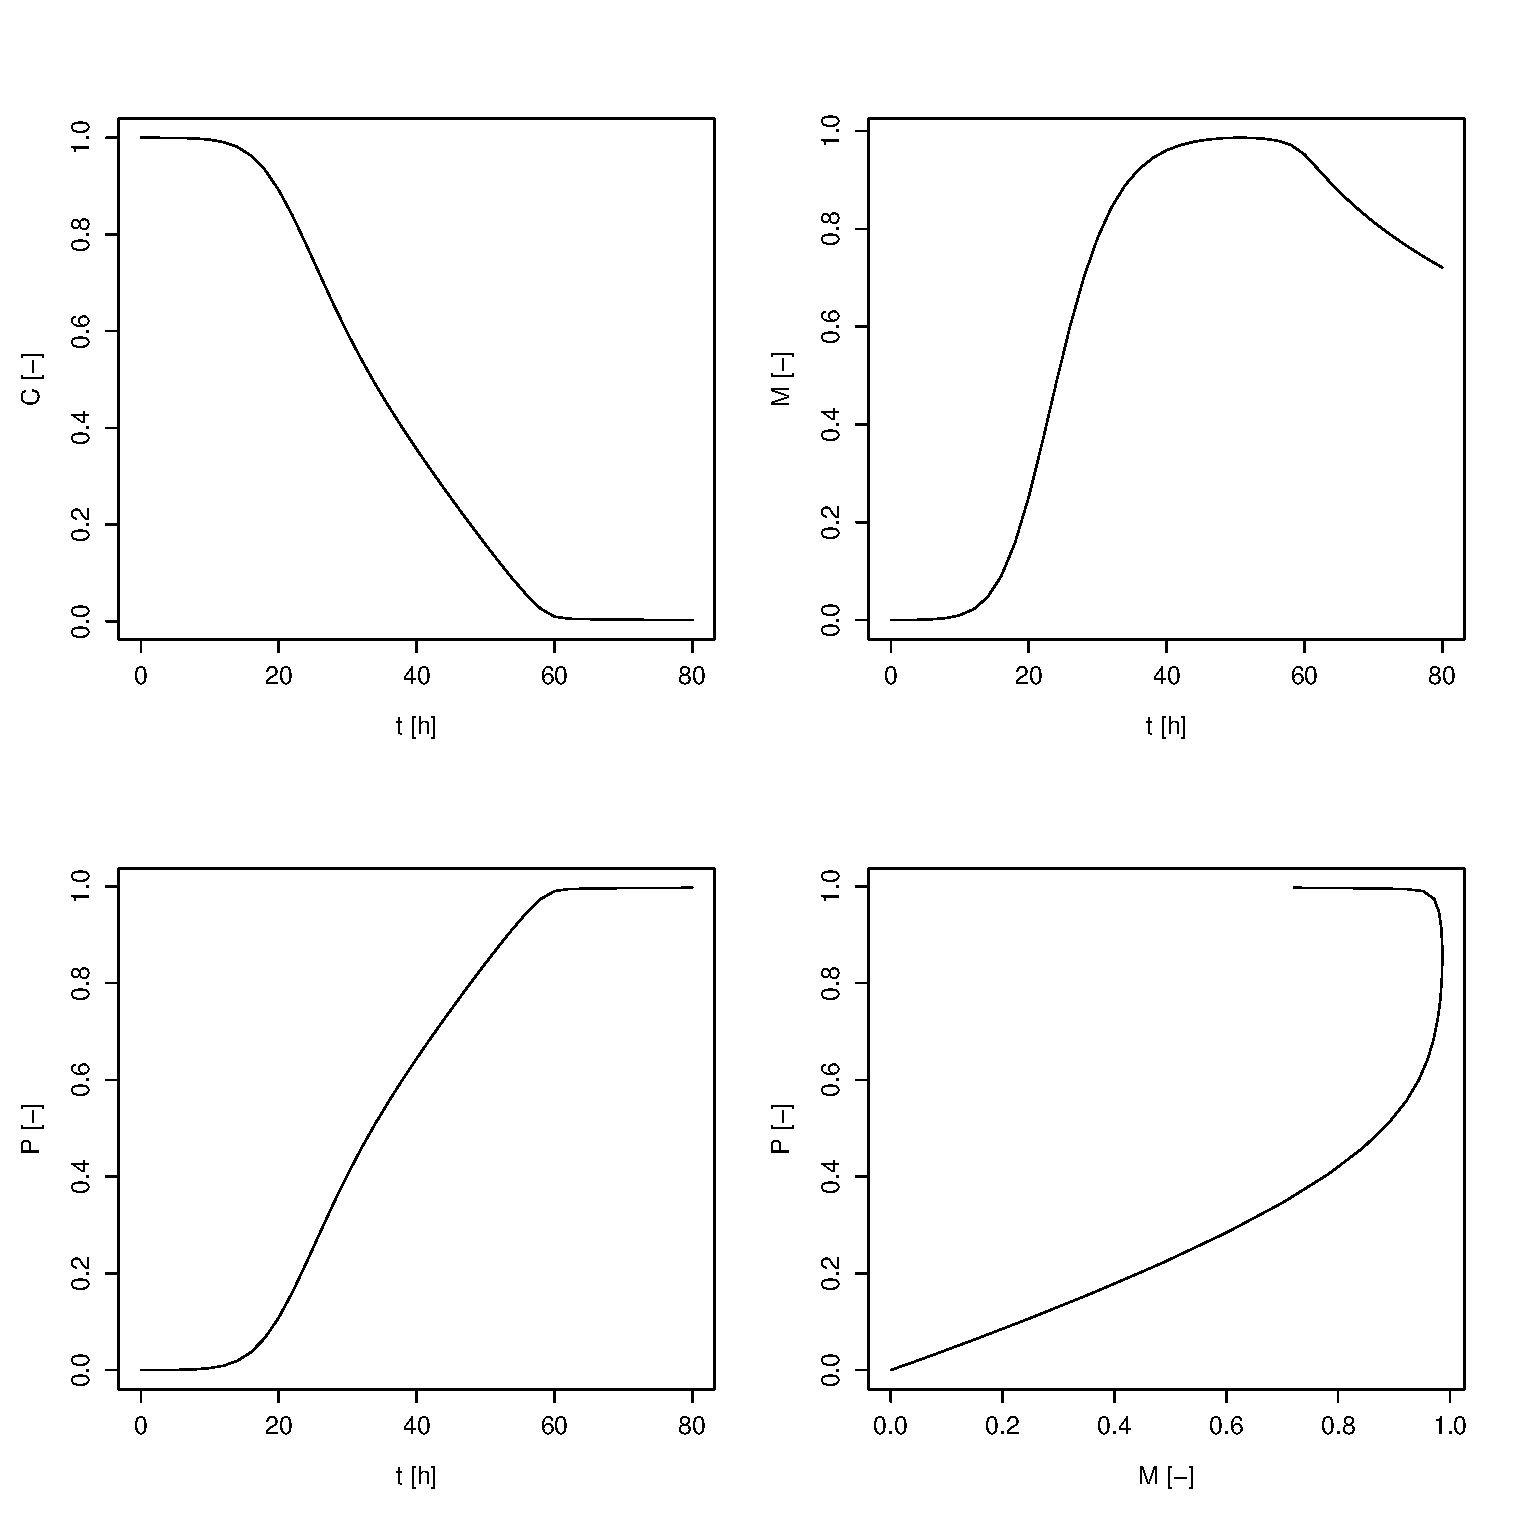
\includegraphics[scale=0.6]{alex_ode_results.eps}
  \caption{A typical model simulation from the simple ODE model.
    Shown are substrate concentration $C$ (top left, normalised), effective sessile biomass $M$ (top right, relative to the ideal carrying capacity $M_{\infty}$), and $CO_2$ product $P$ (bottom left, in moles) as functions of time $t$;.
    Also shown is the product $P$ vs sessile biomass $M$ (bottom right, in moles).
    Figure originally from \cite{dumitrache2015mathematicalModeling}.
  }
  \label{fig:alex_ode_results}
\end{figure}

\subsection{$CO_2$ Production}

Some important quantities to track are the total amount of biomass, $M$, and substrate, $C$. 
%!% HERB: _T_h_e_s_e__v_a_l_u_e_s_ <- Approximations via discretization??
These approximations across the discretization will be called $T_M(t)$ and $T_C(t)$ to represent the total biomass and total substrate, respectively.
The computation for these values can be done by integrating over the region, $\Omega$:
\begin{equation}
  T_M(t) = \int_{\Omega} M dA, \quad T_C(t) = \int_{\Omega} C dA
\end{equation}
These values can be seen in Figure \ref{fig:typical_total} (bd) for $T_M(t)$ and (c) for $T_C(t)$.

\begin{figure}[!htp]
  \centering
  \begin{tabular}{c c}
    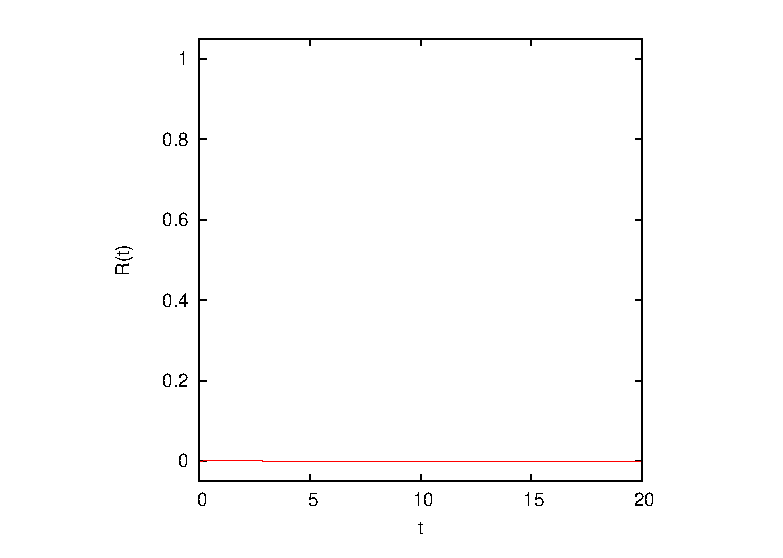
\includegraphics[scale=0.6]{typical_CO2.eps} &
    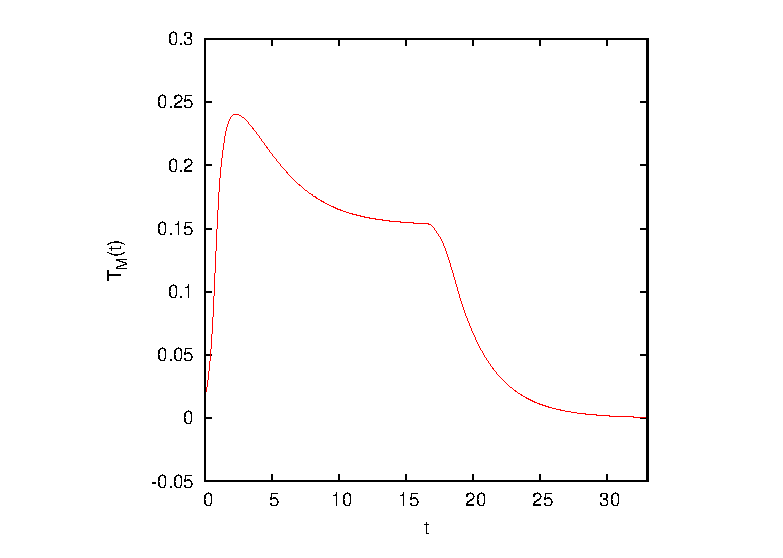
\includegraphics[scale=0.6]{typical_total_M.eps} \\
    (a) & (b) \\
    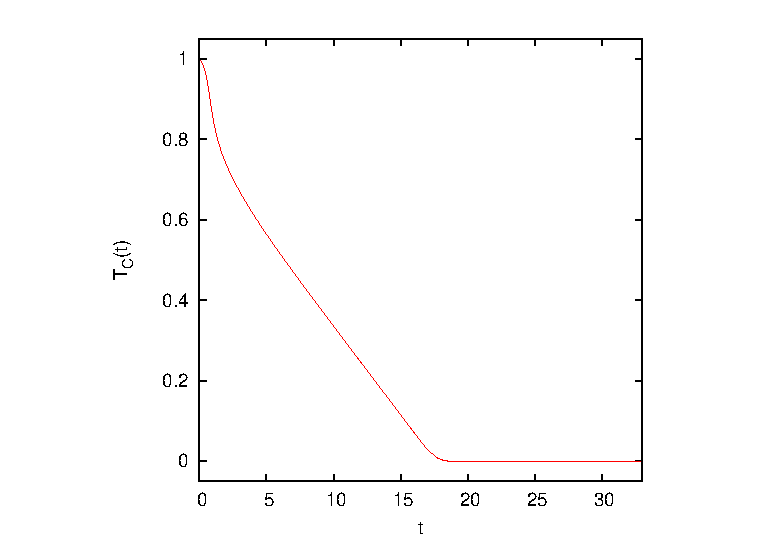
\includegraphics[scale=0.6]{typical_total_C.eps} &
    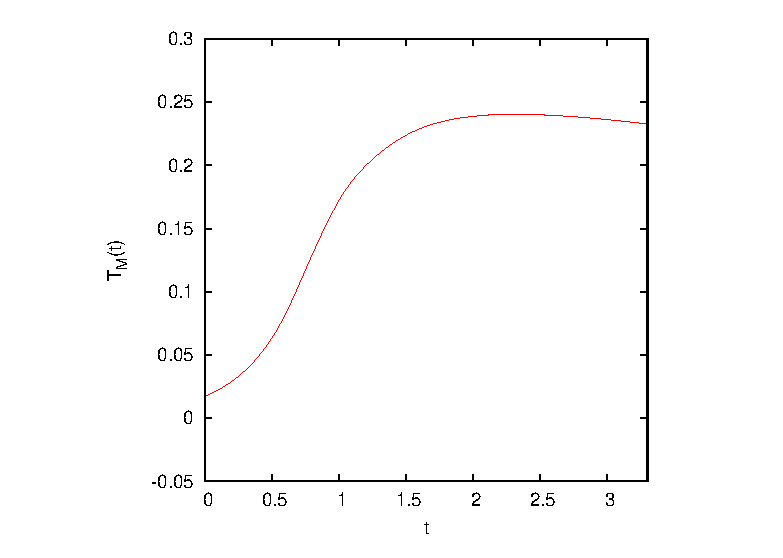
\includegraphics[scale=0.6]{typical_total_M_zoomed.eps} \\
    (c) & (d) \\
    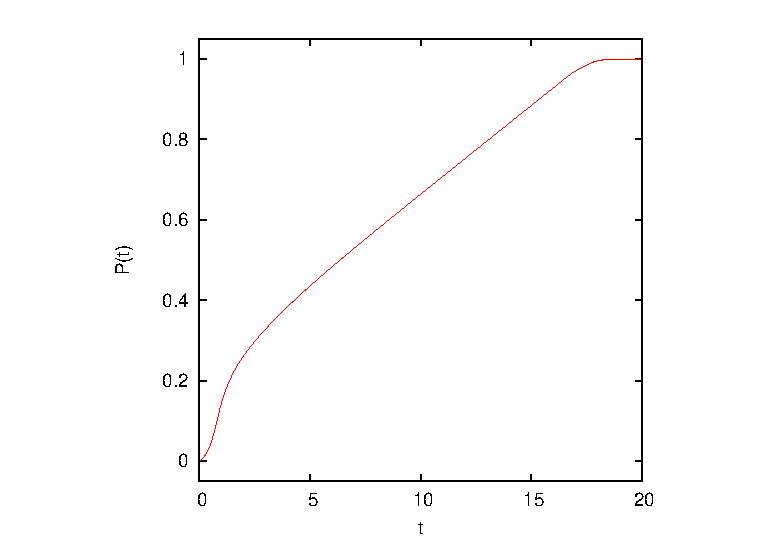
\includegraphics[scale=0.6]{typical_CO2_total.eps} & 
    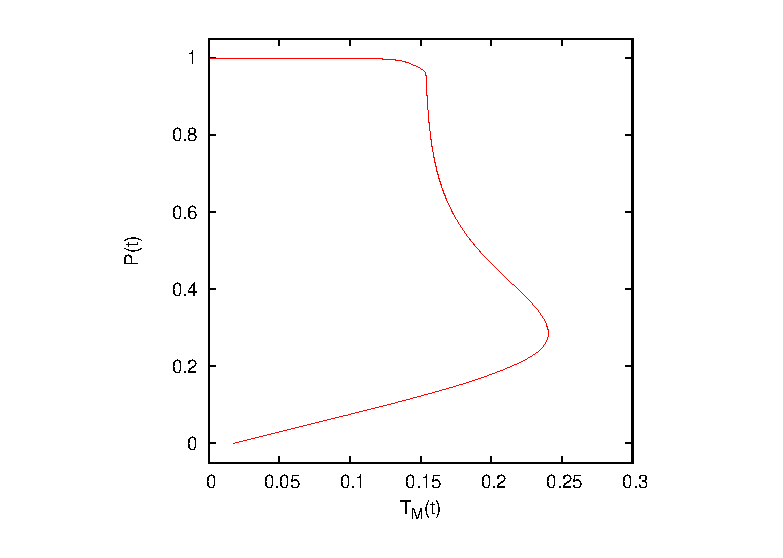
\includegraphics[scale=0.6]{typical_total_PvM.eps} \\
    (e) & (f)
  \end{tabular}
  \caption{Total value of certain qualities from the typical simulation.
    %!% Sometime get this (abcedf) list as an enumerate within the caption... forgot how to do this so look it up later
    Here we have:
    (a) $\mathcal{R}(t)$, the rate of $CO_2$ production,
    (b) total $M$ as a function of time,
    (c) total $C$ as a function of time, 
    (d) total $M$ as a function of time zoomed in from $t = 0$ to $t = 3$,
    (e) $\mathcal{P}(t)$, the total $CO_2$ produced, 
    (f) $\mathcal{P}(t)$ as a function of total $M$.
    All the graphs are from the same simulation with initial condition of $40$ random spherical inoculation points along the $y=0$ side of the region and another $40$ on $y = 1$. 
    A grid of $257 \times 257$ was used for this graph.
    Default parameter set (Appendix A) was used except for $\delta = 10^{-8}$.
  }
  \label{fig:typical_total}
\end{figure}

Since \textit{C. thermocellum} produces $CO_2$ as the substrate is consumed, we can track the production of $CO_2$.
Following the idea from \cite{dumitrache2015mathematicalModeling}, we can equate the change in production of $CO_2$ as time changes by the following equation:
\begin{equation} \label{equ:rho}
p_t = \rho G(C) M.
\end{equation}

To get the amount of $CO_2$ produced at a specific time we get,
\begin{equation}
  \mathcal{R}(t) = \int_\Omega p_t dA = \int_\Omega \rho G(C) M dA.
\end{equation}
From this we can get the more useful value, the total $CO_2$ produced until this point.
\begin{equation}
  \mathcal{P}(t) = \int^t_0 \mathcal{R}(s) ds.
\end{equation}

The $CO_2$ amount is calculated by letting $\rho = 1$ and using the numerically computed values for $G(C)M$ as a measure.
For the same simulation as Figure \ref{fig:typical_sim}, the $CO_2$ information can be seen in Figure \ref{fig:typical_total} (a e).

The results from Figure \ref{fig:typical_total} (c d e f) seems to match the results from the ordinary differential equation model proposed in \cite{dumitrache2015mathematicalModeling}.
Their results can be seen in Figure \ref{fig:alex_ode_results}.
It is important to note that in our system $T_M = 1 $ means that $\Omega$ is completely filled with biomass.
However, in \cite{dumitrache2015mathematicalModeling} they scaled the biomass to the ideal carrying capacity of biomass, i.e. they have $T_M = 1$ when all the biomass is in stage II or III.
The overall result from this experiment is that the spatial two dimension model confirms the conceptual model from \cite{dumitrache2015mathematicalModeling} based on which the reactor-scale model was formulated.
The reactor-scale model consolidated the spatial effects into the carrying capacity of the growth and yet still managed to agree with the results of the actual spatial model.


\section{Travelling Wave Analysis}

%%%%%%%%%%%%%%%%%%%%%%%%%%%%%%%%%%%%%%%%%%%%%%%%%%%%%%%%%%%
\subsection{Spatial Simplification}

To simplify the travelling wave analysis we reduce the spatial dimensions to that of a one dimensional problem.
This can be done if initial conditions that are homogenous with respect to $y$ are chosen.
The purpose of this spatial simplification is that this will speed up the computations considerable.
It will also make visualizations easier as certain figures would become too cluttered in two dimensions.
What is done here is more of a pseudo-reduction of dimensions.
%!% is it n or (n+1) same for m...
By reducing the grids from an $n \times m$ grid to an $n \times 4$ grid we have changed the way the problem size scales with finer grids.
The problem is still two dimensional, just now one dimension has been reduced to only 4 grid points of accuracy instead of $m$ points.
This does not effect the final result since we only apply this change to problems with appropriate initial conditions.
These initial conditions are homogenous in the $y$ direction and thus we do not have any fluctuation between $y$ values for a given $x$ value.

%!% Is it n or (n+1), same for m
One main benefit of changing the grid from $n \times m$ to $n \times 4$ is that the growth of the problem with respect to the resolution of the grid is reduced dramatically.
This changes the problem from a $O(n^2)$ problem to a $O(n)$.
Using the one dimensional travelling wave initial conditions, (\ref{equ:basic_init_trav_wave}), one simulation is computed with a $513 \times 513$ grid, seen at Figure \ref{fig:show_dimension_3D}, and another with a $513 \times 4$ grid, seen at Figure \ref{fig:show_dimension_2D}.

\begin{figure}[!htp]
  \centering
  \begin{tabular}{c c}
    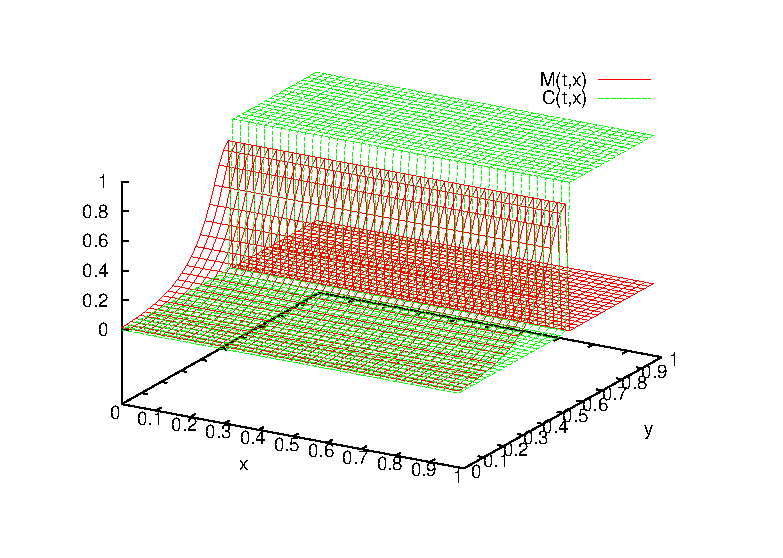
\includegraphics[scale=0.7]{show_dimension_3D.eps} &
    %!% Fix the y axis tics so they don't hidously overlap
    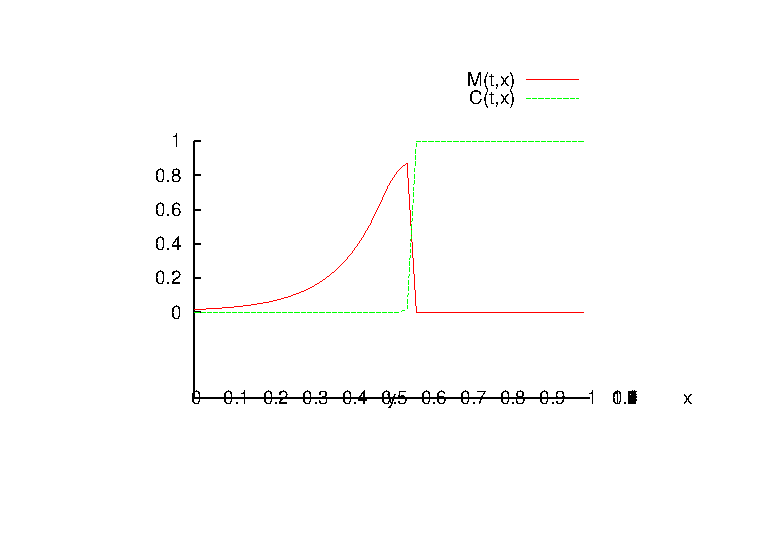
\includegraphics[scale=0.7]{show_dimension_3D_side.eps} \\
    (a) & (b) \\
  \end{tabular}
  \caption{Graph of (a) 3D view of $M(t,x,y)$ and $C(t,x,y)$, (b) Side profile view of $M(t,x,y)$ and $C(t,x,y)$ at $t=40$.} 
  \label{fig:show_dimension_3D}
\end{figure}
   
Before any changes to the grid can be made, it must be confirmed that fluctuations are sufficiently small.
To this end, the standard deviation is used as a measure.
The standard deviation is calculated along the $y$-direction for each x value.
This gives a numerical quantity for the measure of dispersal each $y$ value has with another.
Here, we use the sample standard deviation for the sole reason that this single simulation does not represent its own population.
Initially, at $t =0$ the standard deviation is 0 everywhere (DATA NOT SHOWN).
At $t = 40$, Figure \ref{fig:show_dimension_stddev} show the standard deviation of each $y$ value.
After many time steps have passed the amount of spread is always less then $10^{-14}$, which is an acceptable degree of consistency.
Note that the main inconsistency is at the wave front, around $x = 5.75$, which is mainly because of the sharp change in values.

\begin{figure}[!htp]
  \centering
  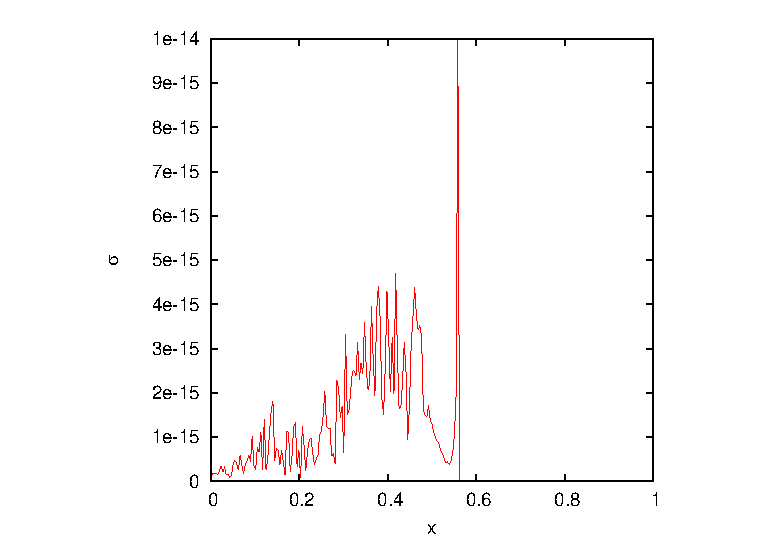
\includegraphics{show_dimension_stddev.eps}
  \caption{The standard deviation at the same time as the above graphs}
  \label{fig:show_dimension_stddev}
\end{figure}

%!% Is it n or n+1?
When simulations are computed with a $n \times 4$ grid, a two dimensional solution is still computed. 
With regards to visualizations, side profiles could be used on these solutions to present pseudo-one dimensional visualizations; this is not ideal.
To visualize the solutions in true one dimension we use $\bar{M}$ and $\bar{C}$ as averaged values of the solutions along the y-axis.
This is computed after the solution has been determined and is independent of the actual computations for M and C.
So by taking the average of the points along the $y$-axis we can get a two dimensional plot as seen in Figure \ref{fig:show_dimension_2D}. 
 
\begin{figure}[!htp]
  \centering
    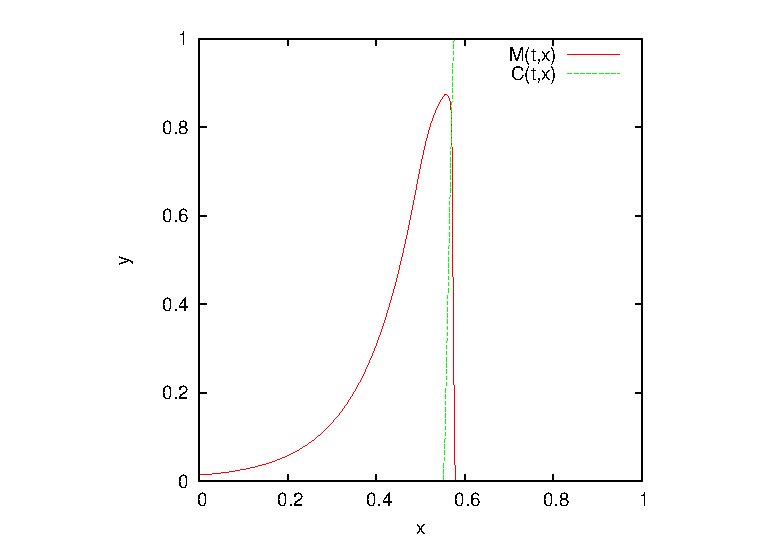
\includegraphics{show_dimension_2D.eps}
    \caption{Graph of M(2,y) and C(2,y), now reduced to a one dimensional solution.}
    \label{fig:show_dimension_2D}
\end{figure}

This means that the system (\ref{equ:model_system}) - (\ref{equ:model_functions}) can be reduced to a one dimensional problem. 
With initial conditions that are homogenous with respect to y, we can greatly reduce the required number of grid points in the one axis.
Once the y-axis reduced, we can also ignore it for visualizations, only using the x-z axis and plotting the values of $\bar{M}$ and $\bar{C}$.


%%%%%%%%%%%%%%%%%%%%%%%%%%%%%%%%%%%%%%%%%%%%%%%%%%%%%%%
\subsection{Travelling Wave Solution}


%!% section 1.2.2 i think before you discuss travelling waves, you should define what they are. Just take it from my old paper
Classical travelling wave solutions are solutions that propagate with an \textit{a priori} unknown constant speed without any change in shape.
This means that the solutions can be defined as 
\begin{equation}
  %!% why \tilde??
  M(t,x) = M(x - ct)
\end{equation}
Figure \ref{fig:trav_wave_solution} shows the time evolution of the single time snapshot from Figure \ref{fig:show_dimension_2D}.
Given the above definition and by looking at the consistent appearance of the solution, it suggests that it is a travelling wave.
It is clear here that the shape of the solution is consistent enough to suggest the existence of a travelling wave solution.

\begin{figure}[!htp]
  \centering
  \begin{tabular}{c c}
      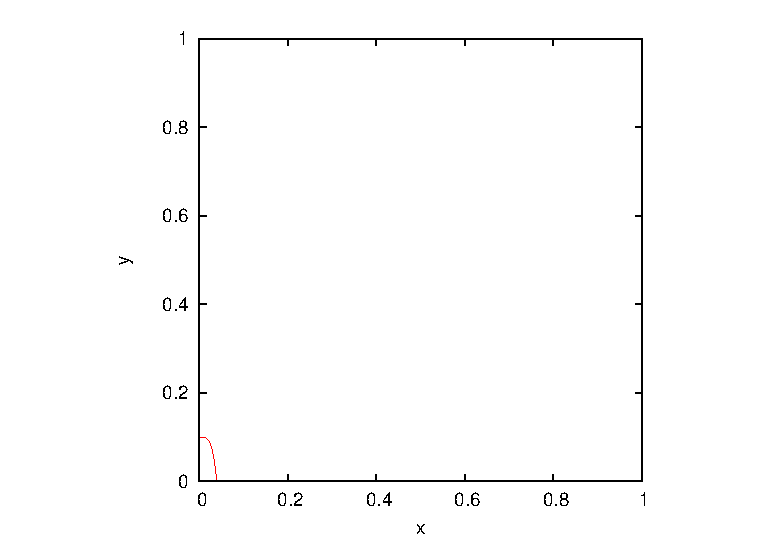
\includegraphics[scale=0.55]{trav_wave_solution_t0.eps} &
      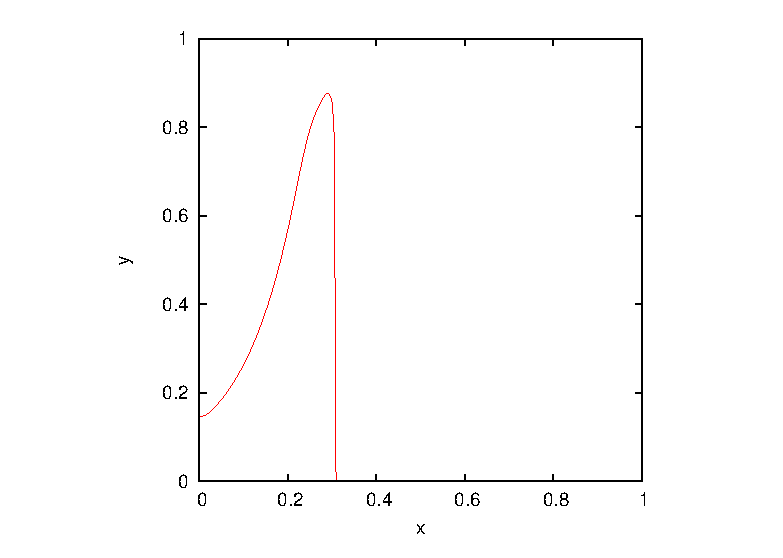
\includegraphics[scale=0.55]{trav_wave_solution_t20.eps} \\
      (a) & (b) \\
      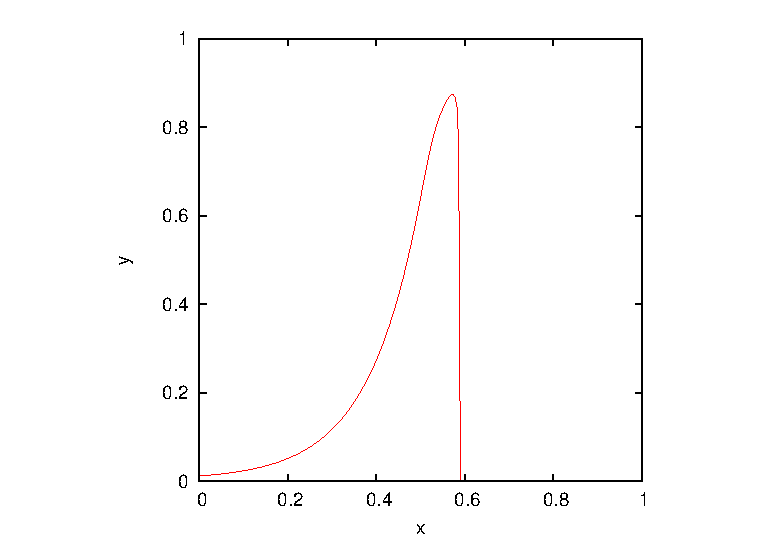
\includegraphics[scale=0.55]{trav_wave_solution_t40.eps} & 
      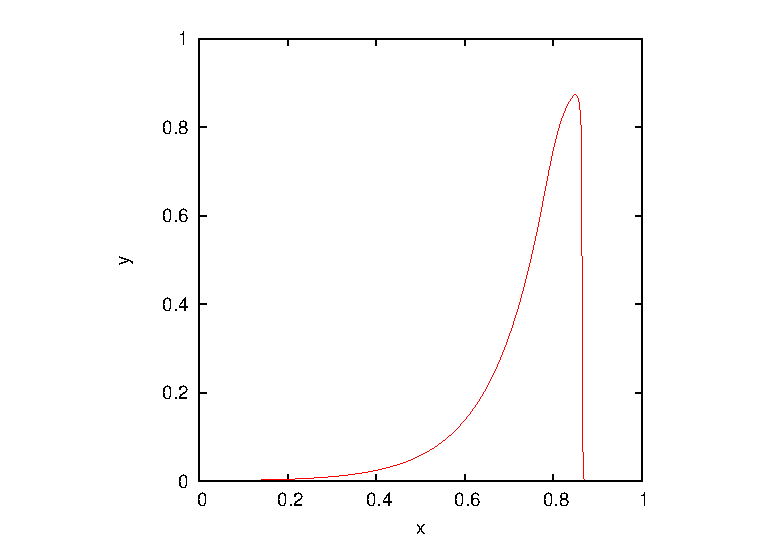
\includegraphics[scale=0.55]{trav_wave_solution_t60.eps} \\
      (c) & (d) 
  \end{tabular}
  \caption{Solutions of $M(x,t)$ and $C(x,t)$ at (a) t = 0, (b) t = 20, (c) = 40, (d) = 60. 
    This was run on a $513 \times 4$ grid.}
  \label{fig:trav_wave_solution}
\end{figure}

The existence of a travelling wave solution for this simulation can be confirmed if the solution $M(x,t)$ can be shown as $M(x-ct)$, where $c$ is the \textit{a priori} unknown wave speed.
This can be graphically confirmed by horizontally translating the solution at different time steps on top of each other.
If the superimposed solutions are of similar shape and have been translated by multiples of the same value then evidence of a travelling wave would be shown.
This would suggest that the value used for horizontal translations is an approximation for the wavespeed $c$. 
We can numerically approximate the value for $c$ by looking at how fast the peak of the wave travels.
The location of the wave peak is the x coordinate that corresponds to the largest $M$ value.
Recall that we are dealing with a pseudo-one dimensional problem, so there does not need to be any consideration for an $(x,y)$ coordinate.
For this case, we used the GNUPLOT software to fit a linear model, $f(x) = mx + b$, to the last half of the wave peaks path, seen in Figure \ref{fig:trav_waveSpeed}.
The last half of the values were used instead of the whole set of values because only for the former do we have a fully formed travelling wave.
The value of $m$ in $f(x)$ is the approximation for the wave speed, $c$. 

\begin{figure}[!htp]
  \centering
    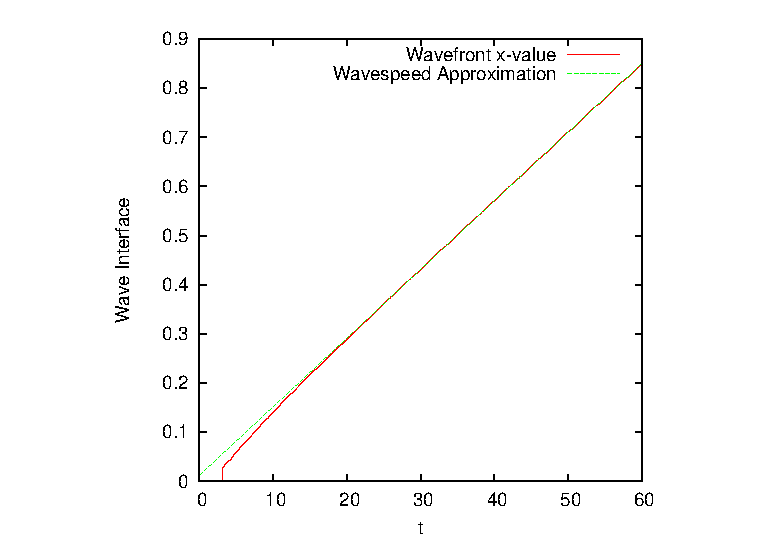
\includegraphics[scale=0.85]{trav_wavespeed.eps}
    %!% At some point, try to get a line in the graphic that show the region that was used for the fitting.
    \caption{The $x$ location of the wave peak as a function of $t$.
      The red line is the wave peak location extracted from the simulation results.
      The green line is the function $f(x) = cx + b$ with c as the wave speed, found by fitting the model to the second half of x values.
      The simulation results used here are from the solution shown in the previous Figure.
    }
    \label{fig:trav_waveSpeed} 
\end{figure}

With an approximation for $c$, the solutions of Figure \ref{fig:trav_wave_solution} can be represented as $M(x - c (t_0 - t_{n}))$, where $t_0 = 60$ is a reference point for the other time steps.
The values of $t_{n}$ are the times for the other solutions.
By translating along the $x$-axis multiple solution profiles can be superimposed, as seen in Figure \ref{fig:trav_wave_translation}.
The shape of each time step is very similar throughout, only differing slightly at the tail.

\begin{figure}[!htp]
  \centering
    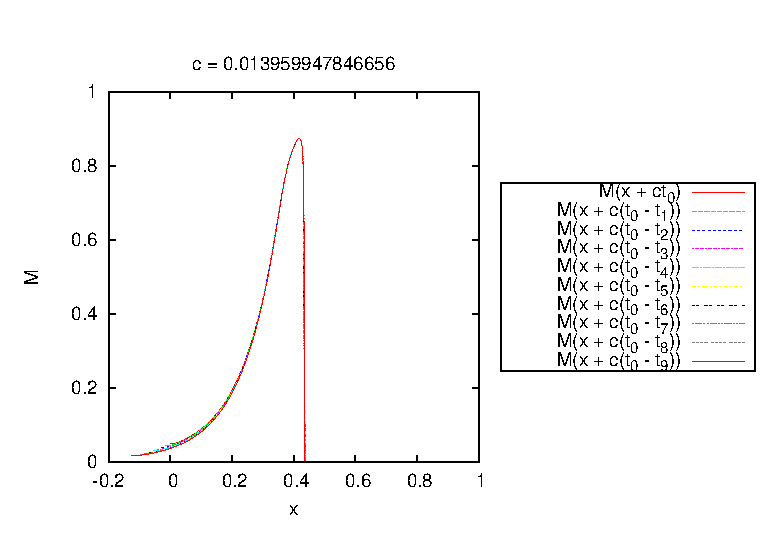
\includegraphics[scale=0.85]{trav_wave_translation.eps}
    \caption{Solutions of $M$ that are represented as $M(x -ct)$ \textit{a priori}.
      The multiple time steps are translated on top of another by horizontal movements of $c (t_0 - t_n)$ for each time step.
      }
    \label{fig:trav_wave_translation}
\end{figure}

Based on the above evidence, we can say that a travelling wave solution has been suggested to exist numerically for a single initial condition and particular set of parameters.
This leads to two logical extensions, looking at the stability of the travelling wave solution based on initial condition and investigating the effect the parameters have on the travelling wave solution.

%%%%%%%%%%%%%%%%%%%%%%%%%%%%%%%%%%%%%%%%%%%%%%%%%%%%%%%%%%%
\subsection{Travelling Wave Stability}

%!% section 4.2.3 not sure that the important thing is really that the wave becomes a 1D solution  ... we can discuss tomorrow or in your exam.
%!% section 1.2.3:  it seems that you are here interested in whether you obtain a 1D travelling wave, i.e. you measure whether your solution deviates from a 1D solution. I am not certain that this is the relevant question. I think the question is whether in a full 2D case you get a travelling wave (which does not need to be a 1D wave but can be a fully 2D solution). Your figure \ref{trav_wavefront} seems to suggest this. We can talk about this in the exam or next week.

Based on the previous example, there seems to exist a travelling wave solution for the intial condition given in (\ref{equ:basic_init_trav_wave}).
The next step is looking at how different initial conditions could still result in a travelling wave solution.
For this we specifically look at the stability of the solution, does it attract each nearby solution into becoming a travelling wave solution or do only special cases become travelling wave solutions.
This will help confirm that the existence of the travelling wave solution is not dependent on the single choice of initial condition.

To test this we take an initial condition that is not inherently one dimensional and see if it approaches the one dimensional property.
The choice of IC is to have multiple random spherical inoculation points along the $y=0$ side of the region.
Specifically, we use $(x_r, y_r)$ to represent the center of each random inoculation point.
Here $x_r \in \mathcal{R}$ and $y_r \in [0, 0.1]$.

The equation used for each random spherical inoculation point is,
\begin{equation}
  M = \frac{-h}{d^2} \left( (x - x_r)^2 + (y - y_r)^2 \right) + h, \quad M \ge  0.
\end{equation}
Random inoculation points add to each other if they overlap.
After all the inoculation points have been generated, every value is divide by the total amount of biomass.
This lets the initial condition become a representation for the distribution of random inoculation points in terms of the total amount generated.
A time evolution of the simulation with the above initial condition can been seen in Figure \ref{fig:trav_stability}.
Here it can be observed that the solution $M$ appears to slowly converge to a one dimensional problem.
This cannot be fully seen since the wave propagation reaches the end of the region before it can become fully one dimensional.

\begin{figure}[!htp]
  \centering
  \begin{tabular}{c c}
      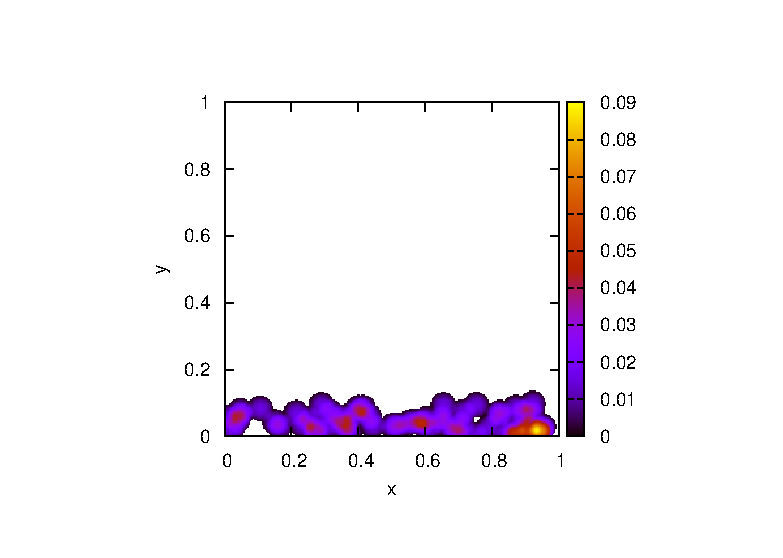
\includegraphics[scale=0.52]{trav_stability_t0.eps} &
      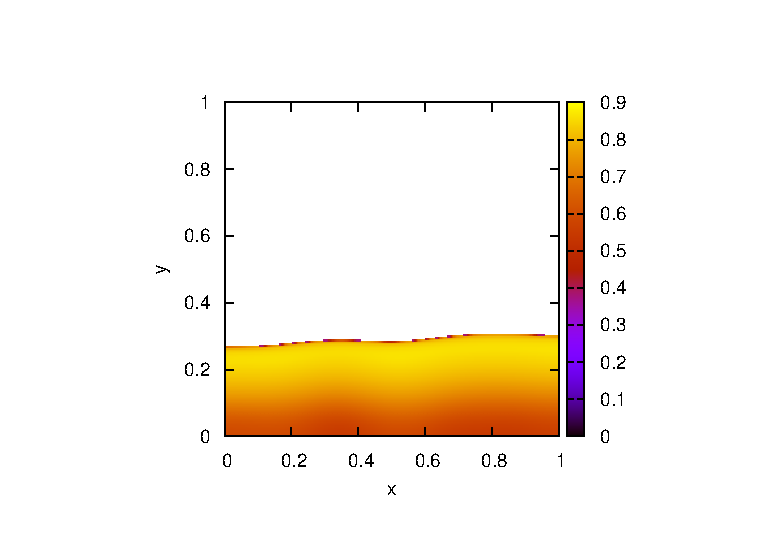
\includegraphics[scale=0.52]{trav_stability_t10.eps} \\
      (a) & (b) \\
      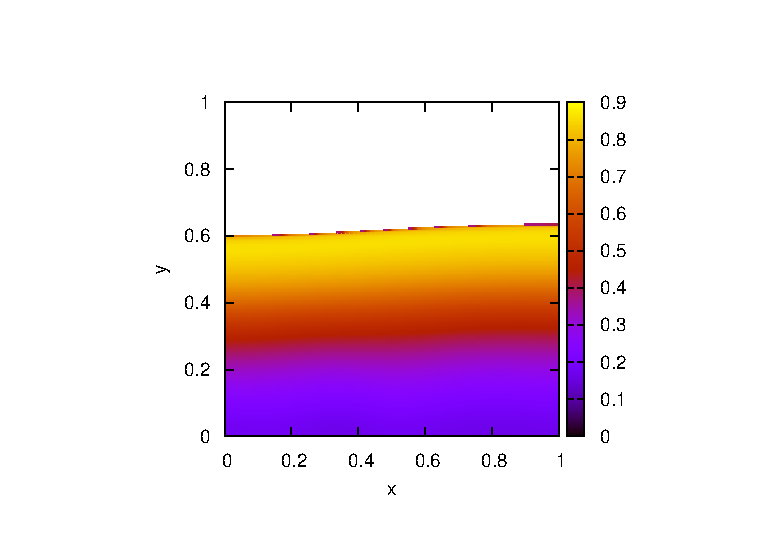
\includegraphics[scale=0.52]{trav_stability_t20.eps} &
      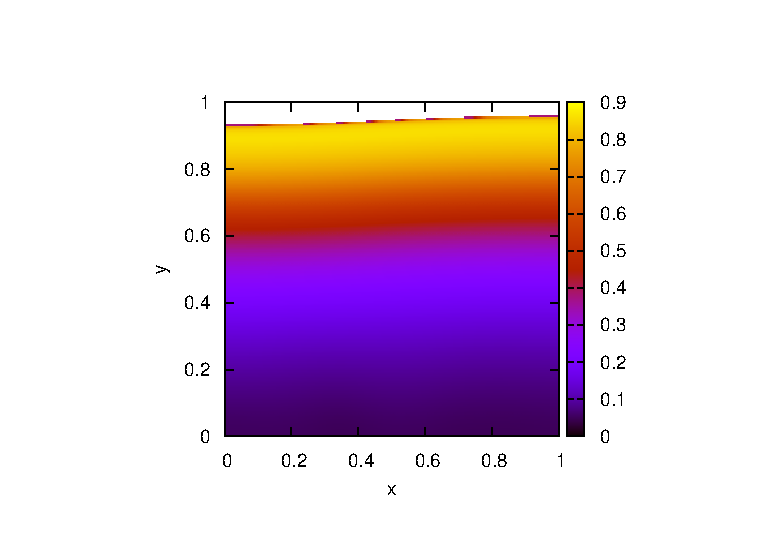
\includegraphics[scale=0.52]{trav_stability_t30.eps} \\
      (c) & (d) 
  \end{tabular}
  \caption{Plots of the simulation with random spherical inoculation points centered in the region $(x,y) \in [0,0] \times [1,0.1]$.
    The solutions are shown at (a) $t = 0$, (b) $t = 10$, (c) $t = 20$, and (d) $t = 30$.
    Each solution is computed on a $513 \times 513$ grid. }
  \label{fig:trav_stability}
\end{figure}

\begin{figure}[!htp]
  \centering
  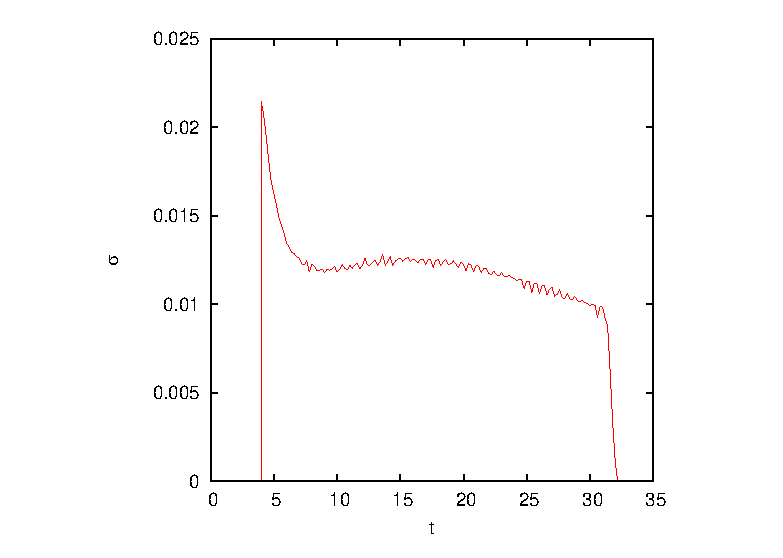
\includegraphics[scale=0.95]{trav_stability.eps}
  \caption{The standard deviation of the wavefront interface as a function of time.
    The wavefront references the largest $y$ coordinate with $M > 0.001$ for each $x$ coordinate.
    The choice of using $M > 0.001$ is because we want to ignore the small values ($~10^{-100}$) that arise from the diffusion right at the wave front. 
    This simulation is the same as the previous Figure.  }
  \label{fig:trav_stability_stddev}
\end{figure}

We can quantitatively see the behaviour of this convergence by calculating the measure of spread at the wave front.
This can be achieved by calculating the standard deviation of $y$ coordinated for each x coordinate.
By tracking the largest $y$ value with a non-zero $M$ for each $x$ value we can generate a sample data set of the wavefront.
The wavefront is used instead of other points of interest, such as the wave peak, because it is the most consistent of characteristics that can be easily tracked.
As seen in Figure \ref{fig:show_dimension_stddev}, the wave peak had the largest spread among all other values. 

\begin{figure}[!htp]
  \centering
  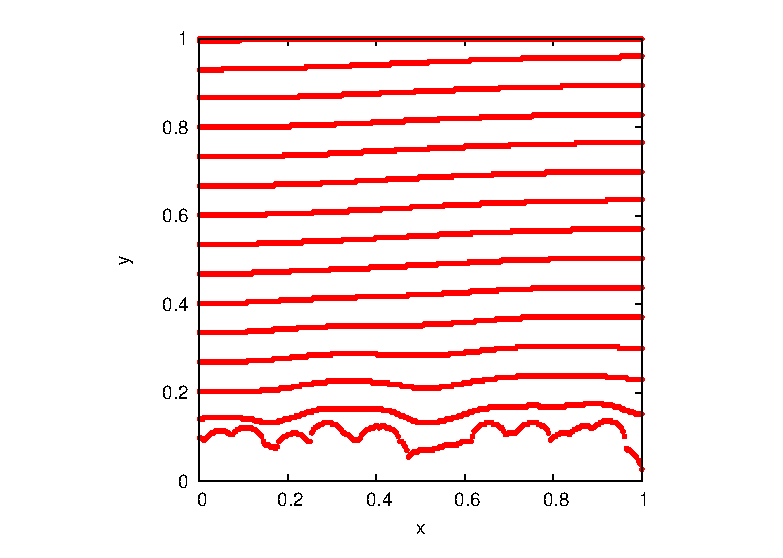
\includegraphics{trav_stability_wavefront.eps}
  \caption{The wavefront shape of multiple time steps.
    Each wavefront has a difference in time by 2, i.e. they are at $t = 4, 6, 8, \ldots, 58, 60$. 
    The simulation results are the same as the previous Figures, using the default parameter values with a grid size $513 \times 513$.
    }
  \label{fig:trav_wavefront}
\end{figure}

Taking the sample standard deviation of this set results in the measure of spread for the wavefront.
The sample standard deviation was used since this one example does not represent the whole population of solutions.
The idea is that, for a solution that converges to one-dimensionality, the $y$ location of the wavefront should be converging to similar values.
This means that the standard deviation would converge to zero.
The standard deviation of the wavefront as a function of time of the simulation ran in Figure \ref{fig:trav_stability} can be seen in Figure \ref{fig:trav_stability_stddev}.
Here is shown that the solution is converging to zero, however not monotonically.
%!% I'm actually not sure what this means.... good news or bad?!

For the numerical computation of the wavefront, the largest $y$ values greater then $0.001$ was used instead of $0$.
The reason is that there are very small values of around $10^{-200}$ that arise due to the diffusion that were not adequate representations of the wavefront.

Another interesting item to investigate is the actual shape of the wavefront.
Figure \ref{fig:trav_wavefront} shows only the wavefront shape for multiple time steps.
The wavefront shape is the same dataset of points used to calculate the standard deviation of the wavefront interface.
Of interest is that the wavefront seems to move at a constant speed, since each wavefront shown is equidistance from the next.


%!% Maybe need to try other types of initial conditions to say this for sure...
% Or maybe just run this same experiment 5 or so times to get a better sample and then just show the stddev of all 5 on a single graph. If they all converge to 0ish then that looks pretty strong.


%%%%%%%%%%%%%%%%%%%%%%%%%%%%%%%%%%%%%%%%%%%%%%%%%%%%%%%%%%%
%!% Here I kinda want to show how the wavespeed dectector script works versus when I use the gnuplot fitting to calculate the wavespeed approximation.
% So here a mention the difference between each calculation and then show the horizontal translation graph for both the script and the fitted wavespeed.
%Show computations for the wave speed

%%%%%%%%%%%%%%%%%%%%%%%%%%%%%%%%%%%%%%%%%%%%%%%%%%%%%%%%%%%
\subsection{Parameter Effect on Wave Speed}

The travelling wave solutions seen before have all existed for a single set of parameters.
Here the four main system parameters, $\delta$, $\kappa$, $\nu$, and $\gamma$ are independently varied and the effect on the travelling wave solutions are observed.
From this we can also see how the wave speed of the travelling wave solution changes as a function of the different model parameters.

\begin{figure}[!htp]
  \centering
  \begin{tabular}{c c}
    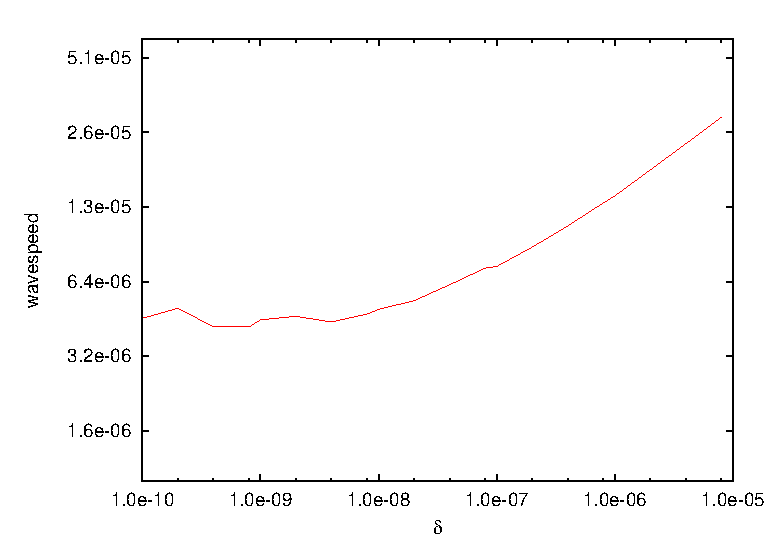
\includegraphics[scale=0.55]{parameter_speed_delta.eps} &
    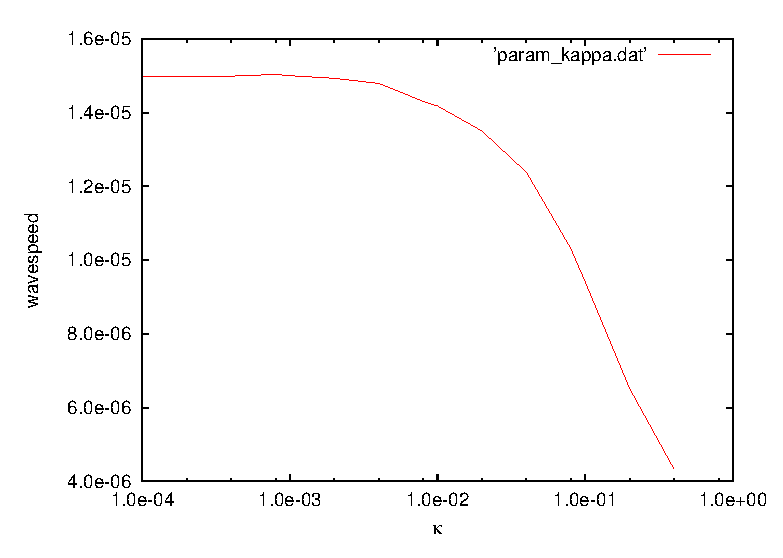
\includegraphics[scale=0.55]{parameter_speed_kappa.eps} \\
    (a) & (b) \\
    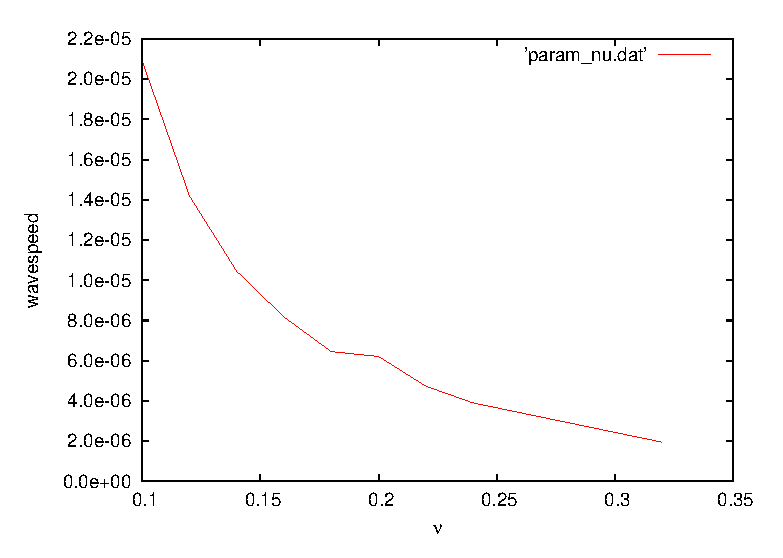
\includegraphics[scale=0.55]{parameter_speed_nu.eps} &
    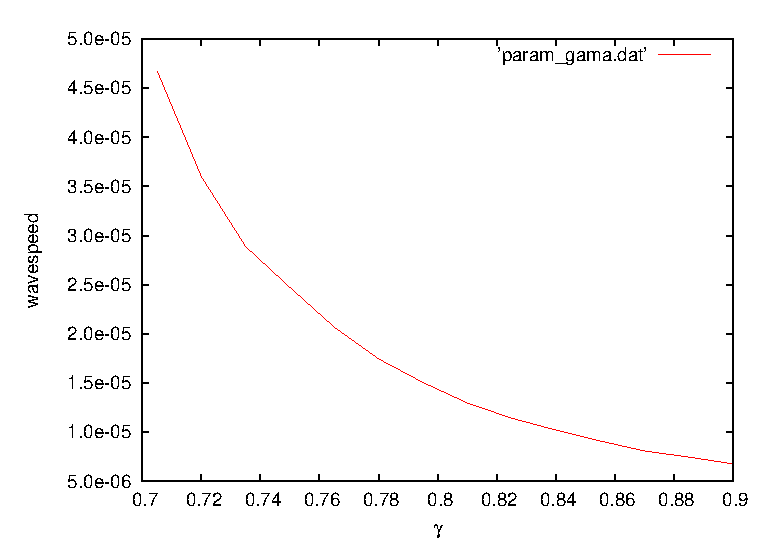
\includegraphics[scale=0.55]{parameter_speed_gama.eps} \\
    (c) & (d) 
  \end{tabular}
  %!% Figure 1.14. the fonts i think are too small; these changes can be made later, not crucial for approving the thesis for defense
  \caption{The value of $c$ as parameter (a) $\delta$, (b) $\kappa$, (c) $\nu$, and (d) $\gamma$ are changed. 
    Note that (a) and (b) have logscales due to the selection of parameter values.
    Each of these were calculated with the same setup as the travelling solution previously done.
    The grid size for each was $513 \times 4$ and a time step of $\Delta t = 0.001$ was used.}
  \label{fig:parameter_speed}
\end{figure}

For this an automated script was created that checks, for each time step, if $M$ is travelling wave solution based on the solution $M$ from a number of time steps previous.
From this check, a wave speed needs to be approximated based on the distance between the two solutions.
If this approximated wave speed is matched throughout all the x values, then a travelling wave solution is assumed to exist at that time step.
With this script, we can try the same simulation as Figure \ref{fig:trav_wave_solution} with different parameter values.

For each parameter, $\delta$, $\kappa$, $\nu$, $\gamma$, the range of values chosen were arbitrarily.
Figure \ref{fig:parameter_speed} shows the results of the wave speed for each parameter changes.
Mainly it was so that the solution did not propagate too fast and hit the end of the region before developing into a full travelling wave solution.
Generally when the travelling wave does not form it is because the wave front propagates to the end of the region faster then the tail of the travelling wave can decrease to 0.
In the case of $\nu$, any larger values than the selected range resulted in biomass that died faster then it could grow, and thus no travelling wave solution exists.
There did not appear to be any cases were a travelling wave solution could not form.

The behaviour of the wave speed as a result of changing the parameters can be explained by the biological meaning of each parameter.
For $\delta$, the diffusion constant, a large value results in a larger local biomass growth as a result of diffusion.
This speeds up the spreading of the biomass and the propagation of the interface.
For $\kappa$, the half-saturation concentration, this value depicts at what substrate concentration we achieve half-maximum growth for the biomass.
When this value is large, the required amount of substrate for optimal growth speed is increased and thus the overall growth of the biofilm is slowed down.
For $\nu$, the decay and loss rate of biomass, a larger value results in more biomass being ejected from the system and thus the amount of biomass available to grow become smaller and growth propagations are slowed.
For $\gamma$, the biomass yield coefficient, a larger value correlates to a substrate that is quickly consumed which produces less total biomass for growth.
This inhibits the propagation of the biomass interface and lowers the wave speed.
The simulated values recorded in Figure \ref{fig:parameter_speed} agree with the expected behaviour for each parameter.




\section{Spatial Effects}

This will be a quick section that goes through:

\begin{itemize}
  \item A quick blerb on what the spatial effects could be and what they can effect. The idea here is that if there are no spatial effects then you can efficently ignore spatial terms and further simplify the model in the future?
  \item Go through the test. Either do two vastly different spatial initial conditions (clumped in a coner vs. uniform distribution). OR the other option (harder but might be cool) is to run many simulations 10+ and show how the total biomass/ wave propgation/ co2 production  changes between them (either it does or doesn't....). Or be really intense and run 30+ simulations and now I have a sample to run statistical analysis on with R.... Not sure about the last one.
  \item Should be a relativly short section.
\end{itemize}

\chapter{Conclusions}
\section{Lessons Learned}

From completing each of the main objectives, some meaningful lessons can be taken from the results:

\begin{itemize}
%  \item What is the main idea of the lesson? From method formulation/validation
%    Where did we learn this from?
%    How does this help things?
  \item From the numerics chapter of the thesis, the validity and usefulness of a newly developed fully-implicit method was investigated.
    By comparing it to the standard semi-implicit method for which it is an extension of it was determined that a significant accuracy gain results from a single extra iteration of the fully-implicit method.
    Multiple iterations increase this gain since the increase in accuracy is positivly correlated to the number of iterations performed.
    However, the computational effort required from the fully-implicit method grows exponentially with higher tolerance.
    The best ratio for solution accuracy when weighed against heavier computation times suggests that two iterations of the fully-implicit method is best (one extra from the semi-implicit method).
    This resulted in an extra digit of accuracy at the cost of approximatly $150\%$ the computational effort.
  \item From the simulation chapter of the thesis, a number of useful characteristics were observed in the system.
    The existance of travelling wave solutions was strongly suggested from all the evidence gathered.
    The stabilty of this wave suggests that it always exists, but this cannot be verified due to the analyitic complexity of the problem.
    Testing two spatially different simulations and measuring the $CO_2$ production showed a large difference between the two solutions at a reactor-scale.
    This suggests that two dimensional models are better for accurately mimicing the behaviour of the system.
\end{itemize}

\section{Future Work}

This will be a quick section.
Mainly have bullet point paragraphs again (like in "lessons learned")
Each bullet paragraph will have:

\begin{itemize}
  \item What could have been changed/improved/explored/avoided?
  \item How could the change be made?
  \item What could this gain?
  \item What possible challenges could this change make?
\end{itemize}

The focus of this section should be for the \textit{non-trivial} points. That is unless it is too difficult to find good points.



\newpage
\pagestyle{References}
\chapter*{References}
\addcontentsline{toc}{chapter}{\hspace{16pt} Bibliography}
\titlespacing{\section}{0pt}{*0}{*0}
\renewcommand{\bibname}{}
\renewcommand\bibsection{}
\titlespacing{\chapter}{0pt}{*0}{*0}
\titlespacing{\section}{0pt}{*0}{*0}
\setlength{\parskip}{0pt}
\setlength{\parsep}{0pt}
\nocite*
\bibliographystyle{apalike}
\bibliography{ThesisReferences}

%\newpage
%\pagestyle{normal}

\appendix
\fancypagestyle{appendix-param}{
\lhead{}
\rhead{\textit{APPENDIX A: DEFAULT PARAMETER VALUES}}
}

\pagestyle{appendix-param}
\chapter{Default Parameter Values}

The default parameter values used for simulation are listed in the follow table. Unless stated, every simulation uses these values.

\begin{table}[h!tb]
  \centering
  \begin{tabular}{| c | c | c |}
    \hline
    Parameter & Symbol & Value \\
    \hline
    - & $\alpha$    & $4$ \\
    - & $\beta$     & $4$ \\
    Decay-Loss rate & $\nu$       & $0.12$ \\
    Half-concentration rate & $\kappa$    & $10^{-3}$ \\
    Yield rate & $\gamma$    & $0.80$ \\
    Diffusion constant & $\delta$    & $10^{-4}$ \\
    \hline
    Initial condition height & $h$ & $0.1$ \\
    Initial condition depth & $d$ & $\frac{5}{127}$ \\
    \hline
    Number of grid points & $nm$ & $513 \times 513$ \\
    Grid size & $\Delta x$  & $\frac{1}{513}$ \\
    Time step & $\Delta t$  & $10^{-3}$ \\
    \hline
  \end{tabular}
  \caption{The listing of default parameter values used for most simulations.}
  \label{tab:default-parameters}
\end{table}


\fancypagestyle{appendix-code}{
\lhead{}
\rhead{\textit{APPENDIX B: SOURCE CODE}}
}

\pagestyle{appendix-code}
\chapter{Source Code}

\lstdefinestyle{mystyle}{
  belowcaptionskip=1\baselineskip,
  xleftmargin=\parindent,
  language=Fortran,
  breaklines=false,
  basicstyle=\footnotesize\ttfamily,
  commentstyle=\itshape\color{BlueViolet},
  stringstyle=\color{black},
  keywordstyle=\bfseries\color{OliveGreen},
  identifierstyle=\color{blue},
  showstringspaces=false,
}

\lstset{style=mystyle}

\singlespacing
\lstinputlisting[language=Fortran, caption=PDE-ODEsolver.f90 main source code]{./Appendix/PDE-ODEsolver.f90}
\doublespacing




%\newpage
%\thispagestyle{custom}
%\mbox{}

\end{document}
